
%----------------------------------------------------------------------------------------
%	PART
%----------------------------------------------------------------------------------------
\part{Capítulo siete}
% \spanishdecimal{.}
\graphicspath{ {7_Capitulo/img/ejemplos/}, {W_Varios/2_Portada_capitulos/} }

%----------------------------------------------------------------------------------------
%	CHAPTER 7
%----------------------------------------------------------------------------------------

\chapterimage{ima2} % Chapter heading image


\chapter{Amortización y Capitalización}

%\begin{center}
%    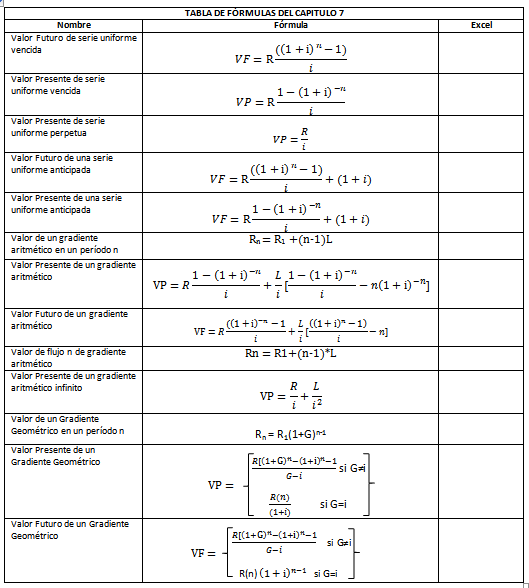
\includegraphics[scale=1]{7_0}
%\end{center}

\section{Mapa Mental}
\begin{center}
	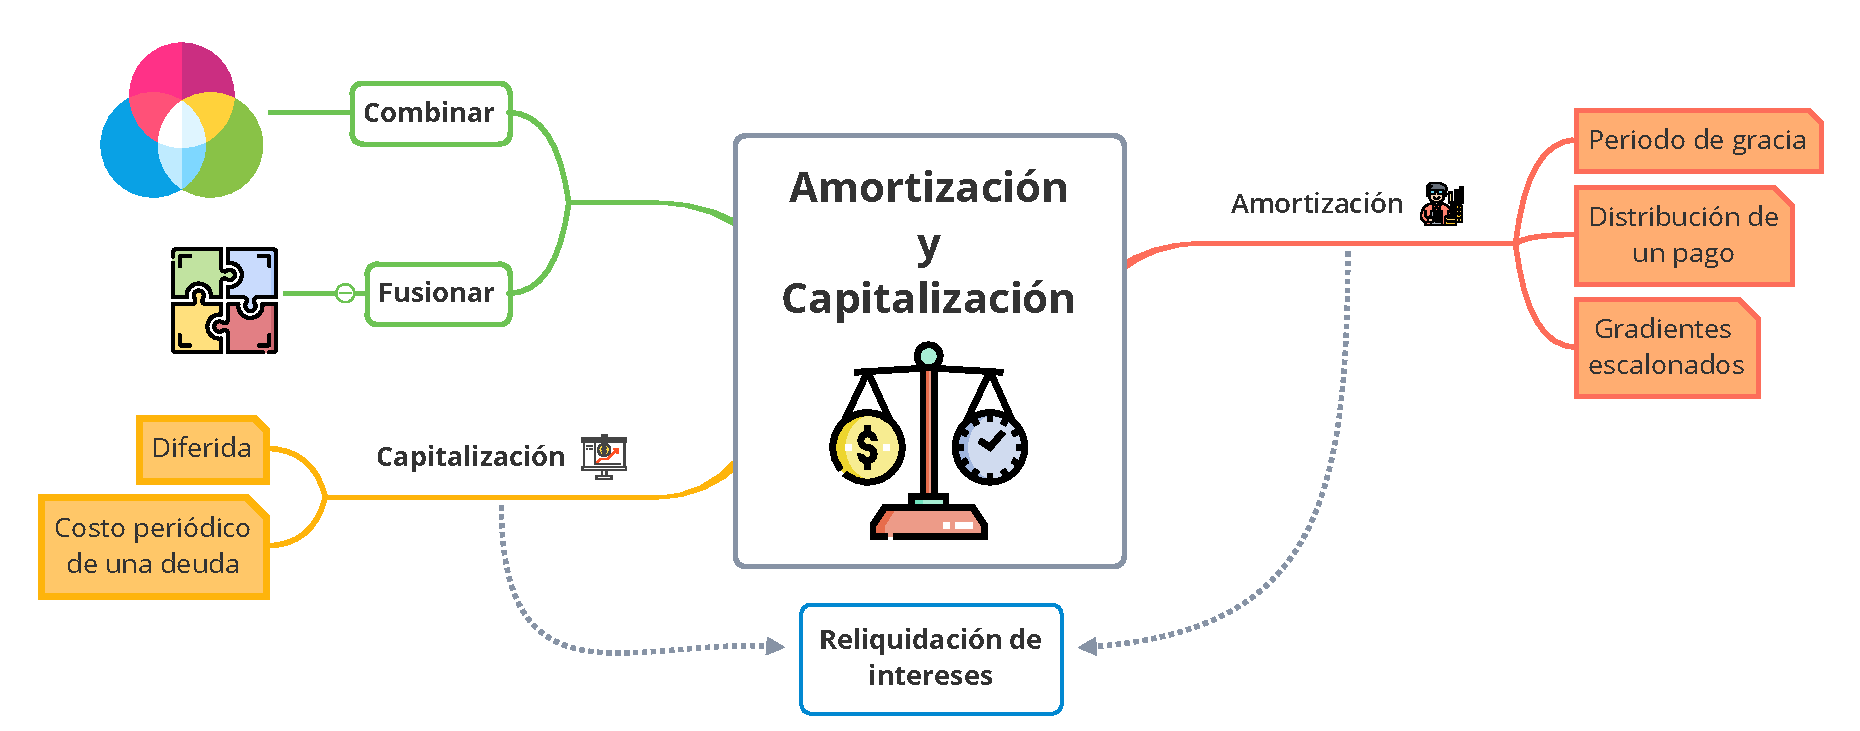
\includegraphics[scale=0.5]{7_Capitulo/img/explicacion/Mapa Mental 7.pdf}
\end{center}

\section{Introducción del capítulo}

Uno de los aspectos más importantes en las finanzas es la AMORTIZACIÓN, porque es la forma más fácil de pagar una deuda; también lo es la CAPITALIZACIÓN, porque así podremos reunir un capital mediante ahorros periódicos. El objetivo en ambos casos viene a ser la financiación de un proyecto. Una manera de visualizar mejor el flujo de caja y el comportamiento de la deuda o del capital a través del tiempo, es mediante el uso de tablas.


\section{Amortización de cuotas con reliquidación de intereses}

Son aquellas en las que deudor y acreedor acuerdan las fechas en que se van a efectuar tales cuotas extraordinarias en el mismo momento en que se contrata el crédito.\\

%Con el siguiente ejemplo analizaremos el valor de la cuota periódica, primero sin cuotas extras (vista en el capítulo 3) y después con cuotas extras pactadas.\\

%%%%%%%%%%% NO OLVIDAR COLOCAR ESTE COMENTARIO CON EL NUMERO DE EJERCICIO %%%%%%%%%%%%%
%%%%%%%%%%%%%%%%%%%% EJERCICIO 1 %%%%%%
%%%Text bf para negrilla , el \\ es para el salto de linea.
%%%El primer \\ hace un espacio en el texto y el 2 \\ crea otro espacio
%\begin{minipage}{\textwidth}
%	\textbf{Ejemplo 1}\newline
%	¿A qué tasa periódica mes vencida,  COP 30{.}000 se convertirán en  COP 35{.}000 en 6 meses?\\ \\
%	\textbf{Solución.}\\
%	\begin{center}
%
%		\renewcommand{\arraystretch}{1.5}% Margenes de las celdas
%		%Creación de la cuadricula
%		\begin{tabular}{|c|c|c| }
%			%Creamos una linea horizontal
%			\hline
%			%Definimos el color de la primera fila
%			\rowcolor[HTML]{FFB183}
%			%%%%% INICIO ASIGNACIÓN FECHA FOCAL %%%%%%%
%			%%%%%%%%%% INICIO TITULO
%			%Lo que se hace aquí es mezclar las 3 columnas en una sola
%			\multicolumn{3}{|c|}{\cellcolor[HTML]{FFB183}\textbf{1. Asignación período focal}}   \\ \hline
%			%%%%%%%%%% FIN TITULO
%			%%%%% INICIO DECLARACIÓN DE VARIABLES %%%%%%%
%			\multicolumn{3}{|c|}{$pf = 6pmv$} \\ \hline
%			%Definimos el color de la primera fila
%			\rowcolor[HTML]{FFB183}
%			%%%%% INICIO DECLARACIÓN DE VARIABLES %%%%%%%
%			%%%%%%%%%% INICIO TITULO
%			\multicolumn{3}{|c|}{\cellcolor[HTML]{FFB183}\textbf{2. Declaración de variables}}                                                                                   \\ \hline
%			%%%%%%%%%% FIN TITULO
%			%%%%%%%%%% INICIO DE MATEMÁTICAS
%			$F =  COP 35\,000$                                                       & $n = 6 \textit{  pmv}$                                                       & $i =  COP ? pmv$ \\
%			$P =  COP 30\,000$                                                       &                                                                              &               \\ \hline
%			%%%%%%%%%% FIN DE MATEMÁTICAS
%			%%%%% FIN DECLARACIÓN DE VARIABLES
%			
%			
%			%%%%% INICIO FLUJO DE CAJA
%			\rowcolor[HTML]{FFB183}
%			\multicolumn{3}{|c|}{\cellcolor[HTML]{FFB183}\textbf{3. Diagrama de flujo de caja}}                                                                                  \\ \hline
%			%Mezclamos 3 columnas y pondremos el dibujo
%			%%%%%%%%%%%%% INSERCIÓN DE LA IMAGEN
%			\multicolumn{3}{|c|}{ 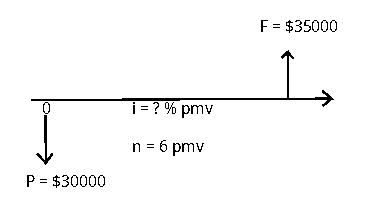
\includegraphics[scale=1.2]{1/capitulo1ejemplo1.pdf} }                                                                                         \\ \hline
%			%%%%%%%%%%%%% FIN INSERCIÓN DE IMAGEN
%			%%%%%FIN FLUJO DE CAJA
%			
%			
%			
%			%%%%% INICIO DECLARACIÓN FORMULAS
%			%%%%%%%%%%% INICIO TITULO
%			\rowcolor[HTML]{FFB183}
%			\multicolumn{3}{|c|}{\cellcolor[HTML]{FFB183}\textbf{4. Declaración de fórmulas}}                                                                                    \\ \hline
%			%%%%%%%%%%% FIN TITULO
%			%%%%%%%%%%% INICIO MATEMÁTICAS
%			
%			$F = P(1+in) \hspace{0.3cm} \textit{Valor futuro}$                   & \multicolumn{2}{c|}{$i = \frac{F}{nP}-\frac{1}{n} \hspace{0.3cm}\textit{Tasa de interés periódica}$}                      \\ \hline
%			%%%%%%%%%% FIN MATEMÁTICAS
%			%%%%%% INICIO DESARROLLO MATEMÁTICO
%			\rowcolor[HTML]{FFB183}
%			%%%%%%%%%%INICIO TITULO
%			\multicolumn{3}{|c|}{\cellcolor[HTML]{FFB183}\textbf{5. Desarrollo matemático}}                                                                                      \\ \hline
%			%%%%%%%%%% FIN TITULO
%			%%%%%%%%%% INICIO MATEMÁTICAS
%			 \multicolumn{3}{|c|}{$i =\frac{ COP 35{.}000}{6\cdot  COP 30{.}000}-\frac{1}{6}=0.2778$}                 \\ \hline
%			%%%%%%%%%% FIN MATEMÁTICAS
%			%%%%%% FIN DESARROLLO MATEMÁTICO
%			
%			\rowcolor[HTML]{FFB183}
%			\multicolumn{3}{|c|}{\cellcolor[HTML]{FFB183}\textbf{6. Respuesta}}    \\ \hline    
%			
%			\multicolumn{3}{|c|}{$i = 2.778\%pmv$} \\ \hline
%		\end{tabular}
%		%Se crean dos lineas en blanco para que no quede el siguiente texto tan pegado
%		\newline \newline
%	\end{center}
%\end{minipage}
%%%%%%%%%%%%%%%%%%%%%%%%%%%FIN EJERCICIO X %%%%%%%%%%%%%%%%%%%%%%%%%%%


\section{Amortización de cuotas sin reliquidación de intereses }
Cuando se está realizando una amortización y el deudor desea hacer un abono extra que no se había convenido en un principio al obtener el crédito, en este caso se dice que la cuota extra es “no pactada”, es apenas lógico, que ésta cuota no aparecerá en la ecuación de valor inicial porque no se había pactado inicialmente y se presentan dos situaciones, la primera opción consiste en abonarlo al saldo de su deuda y dejar que las cuotas ordinarias se sigan haciendo del mismo valor, en este caso la deuda se cancelará antes del plazo previsto, la segunda situación consiste en hacer el abono al saldo de la deuda y efectuar la reliquidación de la cuota ordinaria periódica con el fin de conservar el plazo originalmente pactado, obviamente el valor de la nueva cuota ordinaria será inferior a la liquidada originalmente.
\\\\

%%%%%%%%%% NO OLVIDAR COLOCAR ESTE COMENTARIO CON EL NUMERO DE EJERCICIO %%%%%%%%%%%%%
%%%%%%%%%%%%%%%%%%% EJERCICIO 2 %%%%%%
%%Text bf para negrilla , el \\ es para el salto de linea.
%%El primer \\ hace un espacio en el texto y el 2 \\ crea otro espacio
\textbf{Ejemplo 2}\newline
El jefe de producción de una fábrica debe decidir entre dos máquinas A y B. Las características de cada una son: \\
\begin{center}
		\begin{tabular}{|p{1cm}|p{2cm}|p{2cm}|p{2cm}|p{3cm}|}
			\hline
			\rowcolor{white!50}
			\textbf{Maq.} & \textbf{C} & \textbf{K} & \textbf{S} & \textbf{CAO} \\ \hline
			A            & 800.000 COP   & 3 años     & 200.000 COP    & 25.000 COP       \\ \hline
			B            & 600.000 COP   & 2 años     & 150.000 COP    & 30.000 COP       \\ \hline
		\end{tabular}
\end{center}

Con una tasa del 36\% nominal anual año vencido, determinar la mejor alternativa.

\textbf{Solución.}\\
\begin{center}
	\renewcommand{\arraystretch}{1.5}% Margenes de las celdas
	%Creación de la cuadricula
	\begin{longtable}[H]{|c|c|c|}
		%Creamos una linea horizontal
		\hline
		%Definimos el color de la primera fila
		\rowcolor[HTML]{FFB183}
		%%%%% INICIO ASIGNACIÓN FECHA FOCAL %%%%%%%
		%%%%%%%%%% INICIO TITULO
		%Lo que se hace aquí es mezclar las 3 columnas en una sola
		\multicolumn{3}{|c|}{\cellcolor[HTML]{FFB183}\textbf{1. Asignación período focal}}   \\ \hline
		%%%%%%%%%% FIN TITULO
		%%%%% INICIO DECLARACIÓN DE VARIABLES %%%%%%%
		\multicolumn{3}{|c|}{$pf = 0  \textit{ pav }$} \\ \hline
		%Definimos el color de la primera fila
		\rowcolor[HTML]{FFB183}
		%%%%% INICIO DECLARACIÓN DE VARIABLES %%%%%%%
		%%%%%%%%%% INICIO TITULO
		\multicolumn{3}{|c|}{\cellcolor[HTML]{FFB183}\textbf{2. Declaración de variables}}                                                                                   \\ \hline
		%%%%%%%%%% FIN TITULO
		%%%%%%%%%% INICIO DE MATEMÁTICAS
		$\text{Alternativa A}$ & $\text{Alternativa B}$ & $i= 36\% \text{ pav }$\\
		$C =  800{.}000\text{ COP}$ & $C =  600{.}000\text{ COP}$ & $CPUE =  ?\text{ COP}$\\
		$K =  3 \textit{ años}$ & $K =  2 \textit{ años}$ & \\
		$S =  200{.}000\text{ COP}$ & $S =  150{.}000\text{ COP}$ & \\
		$CAO =  25{.}000\text{ COP}$ & $CAO =  30{.}000\text{ COP}$ & \\
 		$n_{1}= 3 \text{ pav}$ & $n_{2}= 2 \text{ pav}$ &   \\\hline 
		%%%%%%%%%% FIN DE MATEMÁTICAS
		%%%%% FIN DECLARACIÓN DE VARIABLES


		%%%%% INICIO FLUJO DE CAJA
		\rowcolor[HTML]{FFB183}
		\multicolumn{3}{|c|}{\cellcolor[HTML]{FFB183}\textbf{3. Diagrama de flujo de caja}}\\ \hline
		%Mezclamos 3 columnas y pondremos el dibujo
		%%%%%%%%%%%%% INSERCIÓN DE LA IMAGEN
		\multicolumn{3}{|c|}{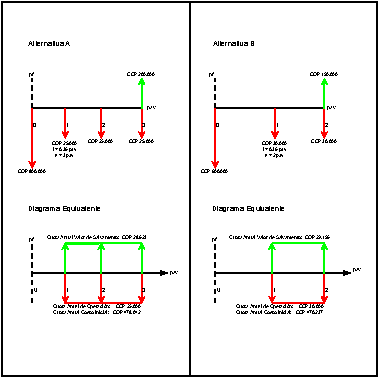
\includegraphics[trim=-5 -5 -5 -5 , scale=2]{10_Capitulo/ejemplos/2/Ejemplo_2.pdf}}
        \\\hline
		%%%%%%%%%%%%% FIN INSERCIÓN DE IMAGEN
		%%%%%FIN FLUJO DE CAJA



		%%%%% INICIO DECLARACIÓN FORMULAS
		%%%%%%%%%%% INICIO TITULO
		\rowcolor[HTML]{FFB183}
		\multicolumn{3}{|c|}{\cellcolor[HTML]{FFB183}\textbf{4. Declaración de fórmulas}} \\ \hline
		%%%%%%%%%%% FIN TITULO
		%%%%%%%%%%% INICIO MATEMÁTICAS

		\multicolumn{3}{|c|}{$VP=R\frac{1-(1+i_{1})^{-n}}{i_{2}} \text{ Valor presente serie uniforme vencida}$}\\ 
		\multicolumn{3}{|c|}{$VF=R\frac{1-(1+i_{1})^{n}}{i_{2}} \text{ Valor futuro aserie uniforme vencida}$}\\\hline
		%%%%%%%%%% FIN MATEMÁTICAS
		%%%%%% INICIO DESARROLLO MATEMÁTICO
		\rowcolor[HTML]{FFB183}
		%%%%%%%%%%INICIO TITULO
		\multicolumn{3}{|c|}{\cellcolor[HTML]{FFB183}\textbf{5. Desarrollo matemático}}   \\ \hline
		%%%%%%%%%% FIN TITULO
		%%%%%%%%%% INICIO MATEMÁTICAS
		Alternativa A & \multicolumn{2}{c|}{Alternativa B}\\ \hline
		Cuota anual costo inicial & \multicolumn{2}{c|}{Cuota anual costo inicial} \\
		${R=\frac{800{.}000}{\frac{1-(1,36)^{-3}}{0,36}} = 178{.}042}\text{ COP}$ & \multicolumn{2}{c|}{${R=\frac{600{.}000}{\frac{1-(1,36)^{-2}}{0,36}} = 470{.}237 }\text{ COP}$} \\
		Cuota anual valor salvamento & \multicolumn{2}{c|}{Cuota anual valor salvamento}\\
		$R=\frac{200{.}000}{\frac{(1,36)^{3}}{0,36}} = 28{.}623\text{ COP} $ & \multicolumn{2}{c|}{$R=\frac{150{.}000}{\frac{(1,36)^{2}}{0,36}} = 29{.}196 \text{ COP}$} \\
		CPUE alternativa A & \multicolumn{2}{c|}{CPUE alternativa B} \\ 
		$CPUE_{A} = 28.623-478.042-25.000 $ & \multicolumn{2}{c|}{$CPUE_{B} = 29.196-470.237-30.000$}\\ 
		$CPUE_{A} = -474.419\text{ COP}$ & \multicolumn{2}{c|}{$CPUE_{B} = -471.04$\text{ COP}}\\
		\hline
		%%%%%%%%%% FIN MATEMÁTICAS
		%%%%%% FIN DESARROLLO MATEMÁTICO

		\rowcolor[HTML]{FFB183}
		\multicolumn{3}{|c|}{\cellcolor[HTML]{FFB183}\textbf{6. Respuesta}}    \\ \hline

		\multicolumn{3}{|c|}{La alternativa que representa menores perdidad es la B.} \\ 
		\hline
	\end{longtable}
	%Se crean dos lineas en blanco para que no quede el siguiente texto tan pegado
	%\newline \newline
\end{center}
%%%%%%%%%%%%%%%%%%%%%%%%%%FIN EJERCICIO X %%%%%%%%%%%%%%%%%%%%%%%%%%%




\section{Amortización con periodos de gracia (*)}
El período de gracia consiste en que, después de efectuado el préstamo, va a pasar cierto tiempo antes de que se empiecen a efectuar pagos y básicamente, existen dos modalidades de préstamo con períodos de gracia:\\

\begin{itemize}
	\item\textbf{ Período de gracia muerto (*):} consiste en que, durante cierto tiempo, no hay pagos de ninguna clase, a este tiempo se le denomina "período de gracia muerto". Lógicamente, esto no se hace gratuitamente, sino que los intereses causados van acumulándose a la deuda; es decir, que durante el período de gracia muerto, la deuda se incrementa. \\
	\item \textbf{Período de gracia con cuota reducida (*):} consiste en que, durante cierto tiempo se pagan unas cuotas reducidas equivalentes al valor de los intereses que se causan, pero sin hacer amortización al capital, en consecuencia, la deuda permanece constante, porque en la medida que se van causando los intereses se van pagando. Este tipo de préstamo está especialmente dirigido al sector industrial y lo denominaremos "período de gracia con cuota reducida". Obviamente, en un mismo préstamo pueden existir las dos modalidades, lo cual puede dar origen a una tercera modalidad. En este caso el período de gracia muerto siempre figurará de primero, le seguirá el período de gracia con cuota reducida y, a continuación, las cuotas ordinarias.\\
\end{itemize}

\textbf{Ejemplo 3}\\
Hallar el valor presente de la siguiente serie con una tasa del 5\% periodo anual mes vencido, utilizando dos formas para resolverlo.\\

%imagen 4
\begin{center}
	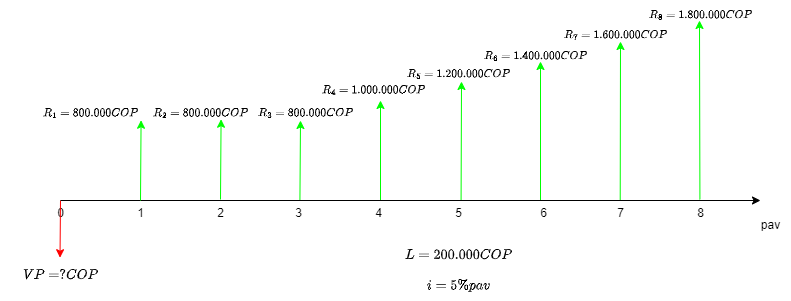
\includegraphics[height=4.0cm]{6_Capitulo/img/ejemplos/6_5}
\end{center}

\textbf{Solución:}

\begin{center}
	\textbf{Primera forma:}
\end{center}

%La tabla ira centrada
\begin{center}
	\renewcommand{\arraystretch}{1.4}% Margenes de las celdas
	%Creación de la cuadricula de 3 columnas
	\begin{longtable}[H]{|c|c|c|}
		%Creamos una linea horizontal
		\hline
		%Definimos el color de la primera fila
		\rowcolor[HTML]{FFB183}
		%%%%% INICIO ASIGNACIÓN PERIODO FOCAL %%%%%%%
		%%%%%%%%%% INICIO TITULO
		%Lo que se hace aquí es mezclar las 3 columnas en una sola
		\multicolumn{3}{|c|}{\cellcolor[HTML]{FFB183}\textbf{1. Asignación período focal}}                                                                                                                            \\ \hline
		\multicolumn{3}{|c|}{$Pf=0 \textit{ pav}$}                                                                                                                                                                    \\ \hline
		%%%%%%%%%% FIN TITULO
		%%%%% INICIO DECLARACIÓN DE VARIABLES %%%%%%%
		%%%%%%%%%% INICIO TITULO
		%Lo que se hace aquí es mezclar las 3 columnas en una sola
		\multicolumn{3}{|c|}{\cellcolor[HTML]{FFB183}\textbf{2. Declaración de variables}}                                                                                                                            \\ \hline
		%%%%%%%%%% FIN TITULO
		%%%%%%%%%% INICIO DE MATEMÁTICAS
		%Cada & hace referencia al paso de la siguiente columna
		\multicolumn{2}{|c|}{$\hspace{2 cm}R=800{.}000 COP \hspace{2 cm}$} & $i=5\%\textit{ pav}$                                                                                                                     \\
		\multicolumn{2}{|c|}{$L=  200{.}000COP$}                           & $n_1=2\textit{ pav}$                                                                                                                     \\
		\multicolumn{2}{|c|}{$VP= ?COP $}                                  & $n_2=6\textit{ pav}$                                                                                                                     \\\hline

		%%%%%%%%%% FIN DE MATEMÁTICAS
		%%%%% FIN DECLARACIÓN DE VARIABLES


		%%%%% INICIO FLUJO DE CAJA
		\rowcolor[HTML]{FFB183}
		\multicolumn{3}{|c|}{\cellcolor[HTML]{FFB183}\textbf{3. Diagrama de flujo de caja}}                                                                                                                           \\ \hline
		%Mezclamos 3 columnas y pondremos el dibujo
		%%%%%%%%%%%%% INSERCIÓN DE LA IMAGEN
		%Deberán descargar las imágenes respectivas del drive y pegarlas en la carpeta
		%n_capitulo/img/ejemplos/1/capitulo1ejemplo1.pdf  (el /1/ es el numero del ejemplo)
		\multicolumn{3}{|c|}{ 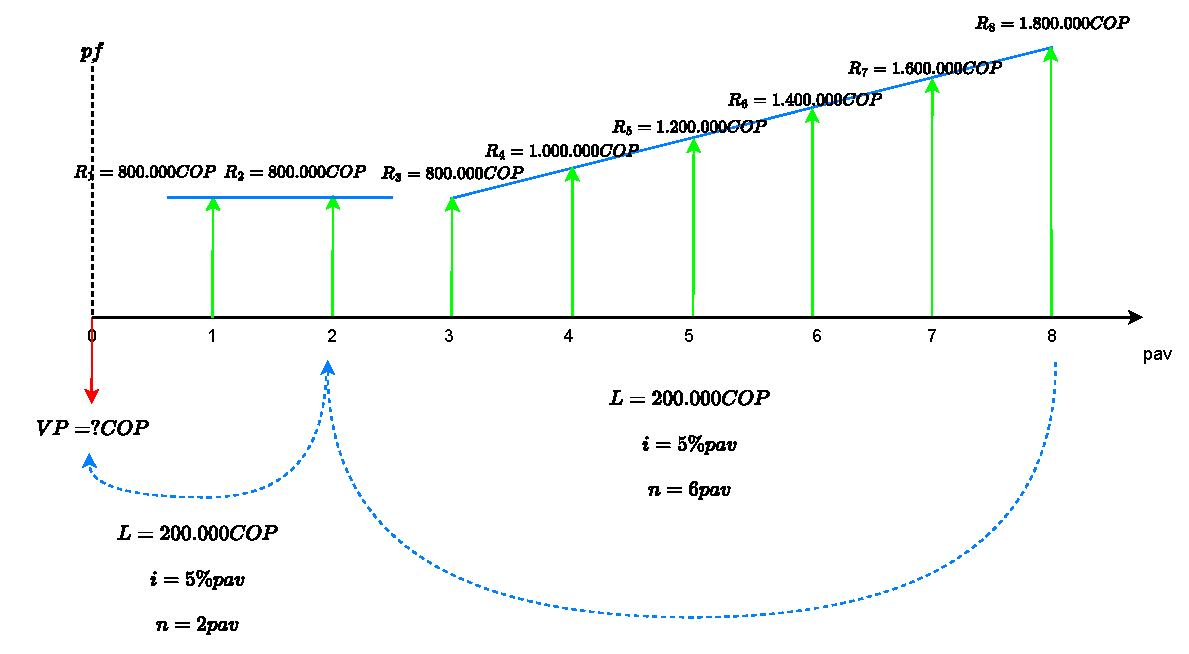
\includegraphics[trim=-5 -5 -5 -5 , scale=0.4]{6_Capitulo/ejemplos/3/Capitulo6Ejemplo3a.pdf} }

		\\ \hline
		%%%%%%%%%%%%% FIN INSERCIÓN DE IMAGEN
		%%%%%FIN FLUJO DE CAJA

		%%%%% INICIO DECLARACIÓN FORMULAS
		%%%%%%%%%%% INICIO TITULO
		\rowcolor[HTML]{FFB183}
		\multicolumn{3}{|c|}{\cellcolor[HTML]{FFB183}\textbf{4. Declaración de fórmulas}}                                                                                                                             \\ \hline
		%%%%%%%%%%% FIN TITULO
		%%%%%%%%%%% INICIO MATEMÁTICAS

		\multicolumn{3}{|c|}{$VP=R(\frac{1-(1+i)^{-n}}{i})+\frac{L}{i}[\frac{1-(1+i)^{-n}}{i}-n(1+i)^{-n}] \hspace{0.4 cm} \textit{Valor presente gradiente aritmético}$}                                             \\
		\multicolumn{3}{|c|}{$VP=R(\frac{1-(1+i)^{-n}}{i}) \hspace{0.4 cm} \textit{Valor presente de una serie unifrome vencida}$}                                                                                    \\
		\multicolumn{3}{|c|}{$P=F(1+i)^{-n} \hspace{0.4 cm} \textit{Valor presente dado un valor futuro}$}                                                                                                            \\ \hline

		%%%%%%%%%% FIN MATEMÁTICAS
		%%%%%% INICIO DESARROLLO MATEMÁTICO
		\rowcolor[HTML]{FFB183}
		%%%%%%%%%%INICIO TITULO
		\multicolumn{3}{|c|}{\cellcolor[HTML]{FFB183}\textbf{5. Desarrollo matemático}}                                                                                                                               \\ \hline
		%%%%%%%%%% FIN TITULO
		%%%%%%%%%% INICIO MATEMÁTICAS
		\multicolumn{3}{|c|}{$VP=  800{.}000COP(\frac{1-(1+0.05)^{-2}}{0.05})+[  800{.}000COP(\frac{1-(1+0.05)^{-6}}{0.05})+\frac{ COP 200{.}000}{0.05}[\frac{1-(1+0.05)^{-6}}{0.05}-6(1+0.05)^{-6}]]$} \\
		\multicolumn{3}{|c|}{$*(1+0.05)^{-2}$}\\
		\multicolumn{3}{|c|}{$VP= 7{.}341{.} \textit{  COP }$}                                                                                                                                                       \\ \hline


		%%%%%%%%%% FIN MATEMÁTICAS
		%%%%%% FIN DESARROLLO MATEMÁTICO
		%%%%%% INICIO RESPUESTA
		\rowcolor[HTML]{FFB183}
		%%%%%%%%%%INICIO TITULO
		\multicolumn{3}{|c|}{\cellcolor[HTML]{FFB183}\textbf{6. Respuesta}}                                                                                                                                           \\ \hline
		%%%%%%%%%% FIN TITULO
		%%%%%%%%%% INICIO RESPUESTA MATEMÁTICA
		\multicolumn{3}{|c|}{\textbf{$\textit{VP= 7{.}341{.}634.83  COP }$}}
		\\ \hline
		%%%%%%%%%% FIN MATEMÁTICAS
		%%%%%% FIN RESPUESTA
	\end{longtable}
	%Se crean dos lineas en blanco para que no quede el siguiente texto tan pegado
	%\newline \newline %USARLO SI CREES QUE ES NECESARIO
\end{center}
%%%%%%%%%%%%%%%%%%%%%%%%%%FIN EJERCICIO 3.1 %%%%%%%%%%%%%%%%%%%%%%%%%%%

\textbf{Segunda forma:}


%La tabla ira centrada
\begin{center}
	\renewcommand{\arraystretch}{1.4}% Margenes de las celdas
	%Creación de la cuadricula de 3 columnas
	\begin{longtable}[H]{|c|c|c|}
		%Creamos una linea horizontal
		\hline
		%Definimos el color de la primera fila
		\rowcolor[HTML]{FFB183}
		%%%%% INICIO ASIGNACIÓN PERIODO FOCAL %%%%%%%
		%%%%%%%%%% INICIO TITULO
		%Lo que se hace aquí es mezclar las 3 columnas en una sola
		\multicolumn{3}{|c|}{\cellcolor[HTML]{FFB183}\textbf{1. Asignación período focal}}                                                                                                                                                            \\ \hline
		\multicolumn{3}{|c|}{$pf=0 \textit{ pav}$}                                                                                                                                                                                                    \\ \hline
		%%%%%%%%%% FIN TITULO
		%%%%% INICIO DECLARACIÓN DE VARIABLES %%%%%%%
		%%%%%%%%%% INICIO TITULO
		%Lo que se hace aquí es mezclar las 3 columnas en una sola
		\multicolumn{3}{|c|}{\cellcolor[HTML]{FFB183}\textbf{2. Declaración de variables}}                                                                                                                                                            \\ \hline
		%%%%%%%%%% FIN TITULO
		%%%%%%%%%% INICIO DE MATEMÁTICAS
		%Cada & hace referencia al paso de la siguiente columna
		\multicolumn{2}{|c|}{$\hspace{2 cm}R=  800{.}000COP\hspace{2 cm}$} & $i=5\%\textit{ pav}$                                                                                                                                                     \\
		\multicolumn{2}{|c|}{$L=  200{.}000COP$}                           & $n_1=3\textit{ pav}$                                                                                                                                                     \\
		\multicolumn{2}{|c|}{$VP=? COP $}                                  & $n_2=5\textit{ pav}$                                                                                                                                                     \\\hline

		%%%%%%%%%% FIN DE MATEMÁTICAS
		%%%%% FIN DECLARACIÓN DE VARIABLES


		%%%%% INICIO FLUJO DE CAJA
		\rowcolor[HTML]{FFB183}
		\multicolumn{3}{|c|}{\cellcolor[HTML]{FFB183}\textbf{3. Diagrama de flujo de caja}}                                                                                                                                                           \\ \hline
		%Mezclamos 3 columnas y pondremos el dibujo
		%%%%%%%%%%%%% INSERCIÓN DE LA IMAGEN
		%Deberán descargar las imágenes respectivas del drive y pegarlas en la carpeta
		%n_capitulo/img/ejemplos/1/capitulo1ejemplo1.pdf  (el /1/ es el numero del ejemplo)
		\multicolumn{3}{|c|}{ 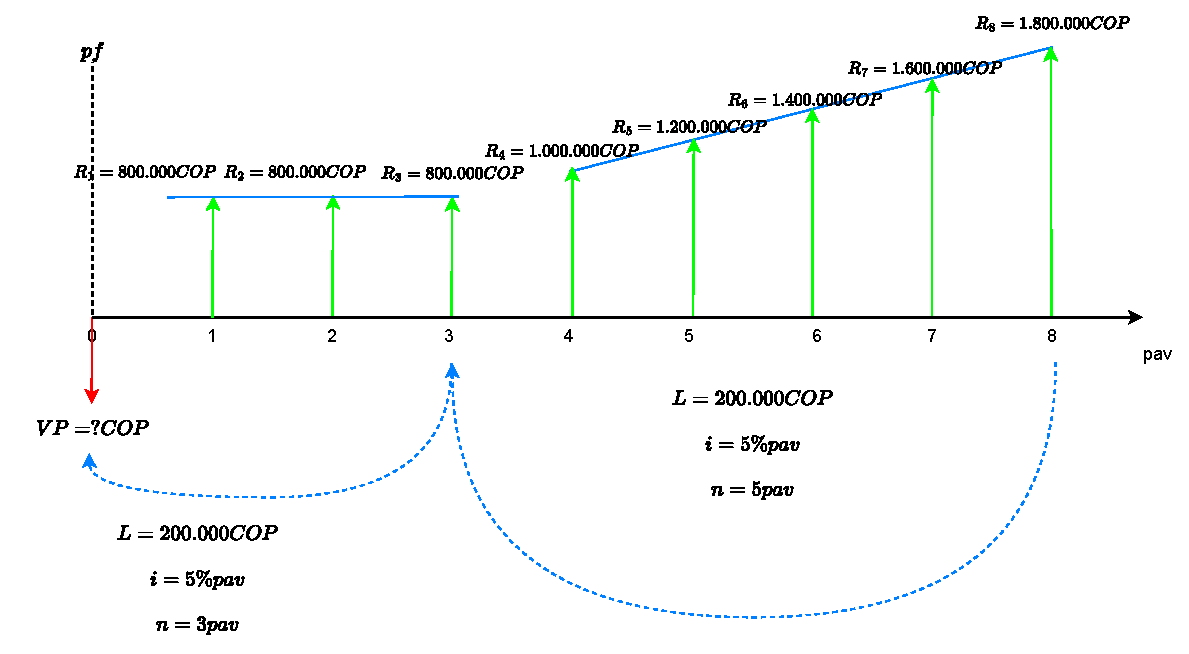
\includegraphics[trim=-5 -5 -5 -5 , scale=0.4]{6_Capitulo/ejemplos/3/Capitulo6Ejemplo3b.pdf} }

		\\ \hline
		%%%%%%%%%%%%% FIN INSERCIÓN DE IMAGEN
		%%%%%FIN FLUJO DE CAJA

		%%%%% INICIO DECLARACIÓN FORMULAS
		%%%%%%%%%%% INICIO TITULO
		\rowcolor[HTML]{FFB183}
		\multicolumn{3}{|c|}{\cellcolor[HTML]{FFB183}\textbf{4. Declaración de fórmulas}}                                                                                                                                                             \\ \hline
		%%%%%%%%%%% FIN TITULO
		%%%%%%%%%%% INICIO MATEMÁTICAS

		\multicolumn{3}{|c|}{$VP=R(\frac{1-(1+i)^{-n}}{i})+\frac{L}{i}[\frac{1-(1+i)^{-n}}{i}-n(1+i)^{-n}] \hspace{0.4 cm} \textit{Valor presente gradiente aritmético}$}                                                                             \\
		\multicolumn{3}{|c|}{$VP=R(\frac{1-(1+i)^{-n}}{i}) \hspace{0.4 cm} \textit{Valor presente de una serie unifrome vencida}$}                                                                                                                    \\
		\multicolumn{3}{|c|}{$P=F(1+i)^{-n} \hspace{0.4 cm} \textit{Valor presente dado un valor futuro}$}                                                                                                                                            \\ \hline

		%%%%%%%%%% FIN MATEMÁTICAS
		%%%%%% INICIO DESARROLLO MATEMÁTICO
		\rowcolor[HTML]{FFB183}
		%%%%%%%%%%INICIO TITULO
		\multicolumn{3}{|c|}{\cellcolor[HTML]{FFB183}\textbf{5. Desarrollo matemático}}                                                                                                                                                               \\ \hline
		%%%%%%%%%% FIN TITULO
		%%%%%%%%%% INICIO MATEMÁTICAS
		\multicolumn{3}{|c|}{$VP=  800{.}000COP(\frac{1-(1+0.05)^{-3}}{0.05})+[  1{.}000{.}000COP(\frac{1-(1+0.05)^{-5}}{0.05})+\frac{  200{.}000COP}{0.05}[\frac{1-(1+0.05)^{-5}}{0.05}-6(1+0.05)^{-6}]]$} \\
		\multicolumn{3}{|c|}{$*(1+0.05)^{-3}\hspace{0.2 cm}\textit{Ec. eqv.}$}\\
		\multicolumn{3}{|c|}{$VP= 7{.}341{.}634 \textit{  COP }$}                                                                                                                                                                                       \\ \hline


		%%%%%%%%%% FIN MATEMÁTICAS
		%%%%%% FIN DESARROLLO MATEMÁTICO
		%%%%%% INICIO RESPUESTA
		\rowcolor[HTML]{FFB183}
		%%%%%%%%%%INICIO TITULO
		\multicolumn{3}{|c|}{\cellcolor[HTML]{FFB183}\textbf{6. Respuesta}}                                                                                                                                                                           \\ \hline
		%%%%%%%%%% FIN TITULO
		%%%%%%%%%% INICIO RESPUESTA MATEMÁTICA
		\multicolumn{3}{|c|}{{$\textit{El valor presente de la serie es  7{.}341{.}634 COP }$}}
		\\ \hline
		%%%%%%%%%% FIN MATEMÁTICAS
		%%%%%% FIN RESPUESTA
	\end{longtable}
	%Se crean dos lineas en blanco para que no quede el siguiente texto tan pegado
	%\newline \newline %USARLO SI CREES QUE ES NECESARIO
\end{center}
%%%%%%%%%%%%%%%%%%%%%%%%%%FIN EJERCICIO 3.2 %%%%%%%%%%%%%%%%%%%%%%%%%%%




La Tabla de Amortización correspondiente es:
\begin{spacing}{1.1}
	\begin{center}
		\begin{tabular}{|p{1cm}|p{2.5cm}|p{2.5cm}|p{2.5cm}|p{3cm}|}
			\hline
			\rowcolor{white!50}
			\textbf{PER\ (1)} & \textbf{SALDO DEUDA (2)=(2)-(5)} & \textbf{INTERESES  (3)=(2)(i)} & \textbf{PAGO\ (4)= R COP - L COP} & \textbf{AMORTIZACIÓN  (5)=(4)-(3)} \\ \hline
			
			0                 &  2.000.000,00 \ COP                  & ---------                       & ---------                   & ---------                          \\ \hline
			1                 &  2.000.000,00 \ COP                   &  220.000,00 \ COP                   & 0,00 \ COP                      &  -220.000,00 \ COP                      \\ \hline
			2                 &  2.464.200,00 \ COP                   &  244.200,00 \ COP                   &  0,00 \ COP                      &  -244.200,00 \ COP                      \\ \hline
			3                 &  2.042.236,06 \ COP                   &  271.062,00 \ COP                    &  693.125,94 \ COP                &  422.063,94 \ COP                       \\ \hline
			4                 &  1.504.332,50 \ COP                   &  224.634,97 \ COP                    &  762.438,53 \ COP                &  537.803,56 \ COP                       \\ \hline
			5                 &  831.126,69 \ COP                     &  165.476,58 \ COP                    &  838.682,39 \ COP                &  673.205,81 \ COP                       \\ \hline
			6                 &  0,00 \ COP                           &  91.423,94 \ COP                     &  922.550,63 \ COP                &  831.126,69 \ COP                       \\ \hline
		\end{tabular}
	\end{center}
\end{spacing}

\textbf{Observación: } La amortización de los períodos 1 y 2 es negativa; esto significa que hay una desamortización o aumento de deuda.\\

\textbf{Ejemplo 4}\\
	Hallar el monto del siguiente flujo de caja que renta una tasa del 15\% periódica año vencido. \\
	\\
	%imagen 5
	\begin{center}
		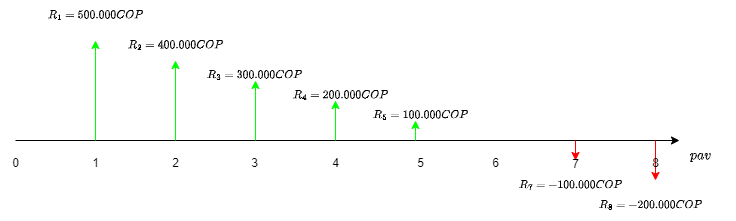
\includegraphics[height=4.5cm]{6_Capitulo/img/ejemplos/6_6}
	\end{center}
	
	\textbf{Solución:}
	
		%La tabla ira centrada
	\begin{center}
		\renewcommand{\arraystretch}{1.4}% Margenes de las celdas
		%Creación de la cuadricula de 3 columnas
		\begin{longtable}[H]{|c|c|c|}
			%Creamos una linea horizontal
			\hline
			%Definimos el color de la primera fila
			\rowcolor[HTML]{FFB183}
			%%%%% INICIO ASIGNACIÓN PERIODO FOCAL %%%%%%%
			%%%%%%%%%% INICIO TITULO
			%Lo que se hace aquí es mezclar las 3 columnas en una sola
			\multicolumn{3}{|c|}{\cellcolor[HTML]{FFB183}\textbf{1. Asignación período focal}}  \\ \hline
			\multicolumn{3}{|c|}{$pf=8 \textit{ pav}$} \\ \hline
			%%%%%%%%%% FIN TITULO
			%%%%% INICIO DECLARACIÓN DE VARIABLES %%%%%%%
			%%%%%%%%%% INICIO TITULO
			%Lo que se hace aquí es mezclar las 3 columnas en una sola
			\multicolumn{3}{|c|}{\cellcolor[HTML]{FFB183}\textbf{2. Declaración de variables}}   \\ \hline
			%%%%%%%%%% FIN TITULO
			%%%%%%%%%% INICIO DE MATEMÁTICAS
			%Cada & hace referencia al paso de la siguiente columna
			\multicolumn{2}{|c|}{$\hspace{2 cm}R=  500{.}000COP\hspace{2 cm}$} & $i=15\%\textit{ pav}$ \\
			\multicolumn{2}{|c|}{$L=-  100{.}000COP$} & $n_1=8\textit{ pav}$ \\ 
			\multicolumn{2}{|c|}{$VF= ?COP $} &  \\\hline
			
			%%%%%%%%%% FIN DE MATEMÁTICAS
			%%%%% FIN DECLARACIÓN DE VARIABLES
			
			
			%%%%% INICIO FLUJO DE CAJA
			\rowcolor[HTML]{FFB183}
			\multicolumn{3}{|c|}{\cellcolor[HTML]{FFB183}\textbf{3. Diagrama de flujo de caja}} \\ \hline
			%Mezclamos 3 columnas y pondremos el dibujo
			%%%%%%%%%%%%% INSERCIÓN DE LA IMAGEN
			%Deberán descargar las imágenes respectivas del drive y pegarlas en la carpeta
			%n_capitulo/img/ejemplos/1/capitulo1ejemplo1.pdf  (el /1/ es el numero del ejemplo)
			\multicolumn{3}{|c|}{ 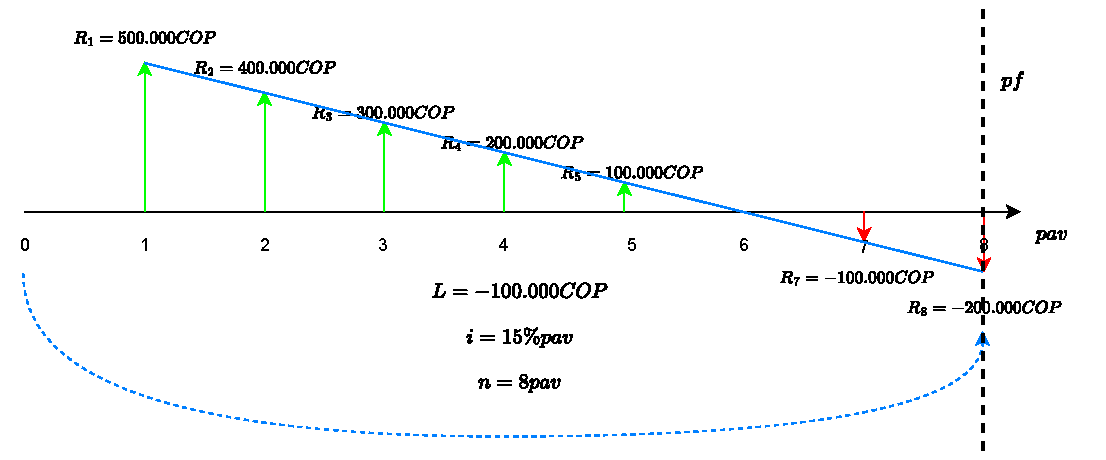
\includegraphics[trim=-5 -5 -5 -5 , scale=0.4]{6_Capitulo/ejemplos/4/Capitulo6Ejemplo4.pdf} }
			
			\\ \hline
			%%%%%%%%%%%%% FIN INSERCIÓN DE IMAGEN
			%%%%%FIN FLUJO DE CAJA
			
			%%%%% INICIO DECLARACIÓN FORMULAS
			%%%%%%%%%%% INICIO TITULO
			\rowcolor[HTML]{FFB183}
			\multicolumn{3}{|c|}{\cellcolor[HTML]{FFB183}\textbf{4. Declaración de fórmulas}}    \\ \hline
			%%%%%%%%%%% FIN TITULO
			%%%%%%%%%%% INICIO MATEMÁTICAS
			
			\multicolumn{3}{|c|}{$VF=R(\frac{(1+i)^{n}-1}{i})+\frac{L}{i}[\frac{(1+i)^{n}-1}{i}-n] \hspace{0.4 cm} \textit{Valor final de gradiente aritmético}$} \\ \hline
			
			%%%%%%%%%% FIN MATEMÁTICAS
			%%%%%% INICIO DESARROLLO MATEMÁTICO
			\rowcolor[HTML]{FFB183}
			%%%%%%%%%%INICIO TITULO
			\multicolumn{3}{|c|}{\cellcolor[HTML]{FFB183}\textbf{5. Desarrollo matemático}}       \\ \hline
			%%%%%%%%%% FIN TITULO
			%%%%%%%%%% INICIO MATEMÁTICAS
			\multicolumn{3}{|c|}{$VF=  500{.}000COP(\frac{(1+0.15)^{8}-1}{0.15})+\frac{-  100{.}000COP}{0.15}[\frac{(1+0.15)^{8}-1}{0.15}-8]\hspace{0.4 cm}\textit{Ecuación de equivalencia}$} \\
			\multicolumn{3}{|c|}{$VF=  3{.}045{.}000 \textit{  COP }$} \\ \hline
			
			
			%%%%%%%%%% FIN MATEMÁTICAS
			%%%%%% FIN DESARROLLO MATEMÁTICO
			%%%%%% INICIO RESPUESTA
			\rowcolor[HTML]{FFB183}
			%%%%%%%%%%INICIO TITULO
			\multicolumn{3}{|c|}{\cellcolor[HTML]{FFB183}\textbf{6. Respuesta}}   \\ \hline
			%%%%%%%%%% FIN TITULO
			%%%%%%%%%% INICIO RESPUESTA MATEMÁTICA
			\multicolumn{3}{|c|}{{$\textit{El monto o valor final del flujo de caja es  3{.}045.000  COP }$}}
			\\ \hline
			%%%%%%%%%% FIN MATEMÁTICAS
			%%%%%% FIN RESPUESTA
		\end{longtable}
		%Se crean dos lineas en blanco para que no quede el siguiente texto tan pegado
		%\newline \newline %USARLO SI CREES QUE ES NECESARIO
	\end{center}
	%%%%%%%%%%%%%%%%%%%%%%%%%%FIN EJERCICIO 4 %%%%%%%%%%%%%%%%%%%%%%%%%%%

	
	\section{Distribución de un pago}
	
	Cada cuota de amortización está compuesta de dos partes: la que corresponde a intereses y la que corresponde a amortización; sin embargo, no es necesario construir la tabla para establecer la proporción en que una cuota dada se divide entre interés y amortización. Basta con calcularle los intereses al capital insoluto del período inmediatamente anterior y luego, restárselo al valor de la cuota, para conocer la parte que corresponde a la amortización. \\
	
	\textbf{Ejemplo 5}\\
Hallar el monto, el valor futuro y el valor presente de 20 pagos de 200.000 COP cada uno, suponga una tasa del 24\% nominal anual año vencido.\\ \\
%\newpage %USAR SOLO SI EL SOLUCIÓN QUEDA SOLO Y ES NECESARIO BAJARLO A LA SIGUIENTE PAGINA
\textbf{Solución.}
%La tabla ira centrada
\begin{center}
 \renewcommand{\arraystretch}{1.5}% Margenes de las celdas
 %Creación de la cuadricula de 3 columnas
 \begin{longtable}[H]{|p{0.333\linewidth}|p{0.3333\linewidth}|p{0.3333\linewidth}|}
  \hline
  \multicolumn{3}{|c|}{\cellcolor[HTML]{FFB183}\textbf{1. Declaración de variables}}                   \\ \hline
  $R= 200.000 COP$         & $i=24\% \hspace{1mm} pav$ & $VP = ? COP$                                  \\
  $n=20 \hspace{1mm} pav$ &                            & $VF= ? COP$                                   \\ \hline
  \multicolumn{3}{|c|}{\cellcolor[HTML]{FFB183}\textbf{2. Tabla de flujo de caja}}                     \\ \hline
  \multicolumn{3}{|p{\columnwidth}|}{
  \begin{center}
   \begin{tabular}{ |p{3.5cm}| p{3cm}|}
    \hline

    \textbf{Periodo (psv) } & \textbf{Flujo} \\ \hline
    0                       & -              \\\hline
    1                       &  200.000 COP     \\ \hline
    2                       &  200.000 COP     \\ \hline
    3                       &  200.000 COP     \\ \hline
    4                       &  200.000 COP     \\ \hline
    5                       &  200.000 COP     \\ \hline
    6                       &  200.000 COP     \\ \hline
    7                       &  200.000 COP     \\ \hline
    8                       &  200.000 COP     \\ \hline
    9                       &  200.000 COP     \\ \hline
    10                      &  200.000 COP     \\ \hline
    11                      &  200.000 COP     \\ \hline
    12                      &  200.000 COP     \\ \hline
    13                      &  200.000 COP     \\ \hline
    14                      &  200.000 COP     \\ \hline
    15                      &  200.000 COP     \\ \hline
    16                      &  200.000 COP     \\ \hline
    17                      &  200.000 COP     \\ \hline
    18                      &  200.000 COP     \\ \hline
    19                      &  200.000 COP     \\ \hline
    20                      &  200.000 COP     \\ \hline
   \end{tabular}

  \end{center}
  }                                                                                                   \\ \hline
  \multicolumn{3}{|c|}{\cellcolor[HTML]{FFB183}\textbf{3. Fórmulas utilizadas}}                       \\ \hline
  \multicolumn{3}{|p{\columnwidth}|}{Mediante el uso de Excel:
  \begin{itemize}
   \item VA (Valor actual): Devuelve el valor presente para una inversión
   \item VF (Valor Futuro): Devuelve el valor futuro de una inversión basado en pagos
         periódicos y constantes, y una tasa de interés constante
  \end{itemize}
  }                                                                                                   \\ \hline
  \multicolumn{3}{|c|}{\cellcolor[HTML]{FFB183}\textbf{4. Desarrollo en Excel}}                       \\ \hline
  \multicolumn{3}{|l|}{Se aplicarán las funciones VA y VF de la siguiente forma:}                     \\
  \multicolumn{3}{|c|}{ 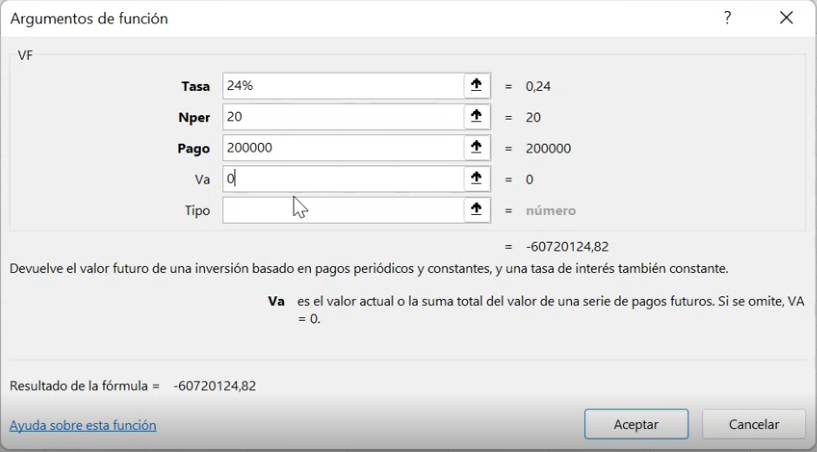
\includegraphics[trim=-5 -5 -5 -5 ,width=1\columnwidth]{5/Ejem5.1.PNG}}        \\
  \multicolumn{3}{|l|}{=VF(0,24;20;-200000;0) con referencia en la hoja de Excel usada para el ejercicio.}    \\
  \multicolumn{3}{|c|}{ 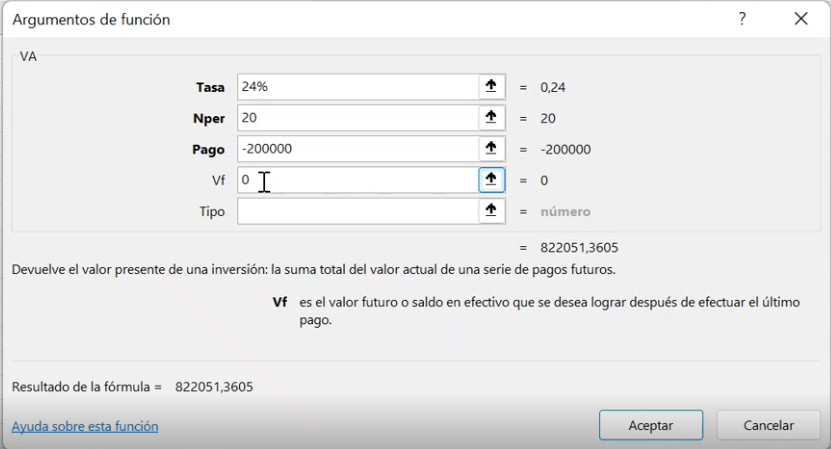
\includegraphics[trim=-5 -5 -5 -5 ,width=1\columnwidth]{5/Ejem5.2.PNG}}        \\
  \multicolumn{3}{|l|}{=VA(0,24;20;-200000;0) con referencia en la hoja de Excel usada para el ejercicio.} \\ \hline
  \multicolumn{3}{|c|}{\cellcolor[HTML]{FFB183}\textbf{5. Respuesta}}                                 \\ \hline
  \multicolumn{3}{|p{\columnwidth}|}{
  El valor presente (VP) o valor actual (VA) es 822.051 COP y el valor futuro (VF) es 60.720.114 COP 
  }                                                                                                   \\ \hline
  \multicolumn{3}{|c|}{\cellcolor[HTML]{FFB183}\textbf{6. Gráfica}}                                   \\ \hline
  \multicolumn{3}{|c|}{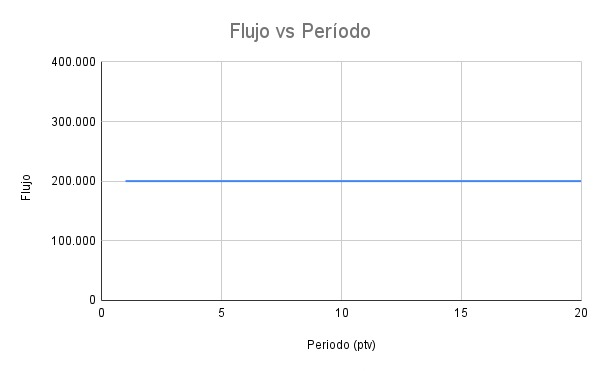
\includegraphics[trim=-5 -5 -5 -5 ,width=0.7\columnwidth]{4/flujovsperiodo.png}}      \\ \hline
 \end{longtable}
 %\newline \newline %USARLO SI CREES QUE ES NECESARIO
\end{center}

 
		
	\textbf{Ejemplo 6}\\
	Calcular el valor presente de una serie infinita de egresos que crecen en  10{.}000COP, si el primer egreso es de  200{.}000COP y la tasa es del 3\% periódica mes vencido.\\
	
	\newpage
	
	%%%%%%%%%%%%%%%%%%% EJERCICIO 6 %%%%%%
	
	%\newpage %USAR SOLO SI EL SOLUCIÓN QUEDA SOLO Y ES NECESARIO BAJARLO A LA SIGUIENTE PAGINA
	\textbf{Solución.}\\
	%La tabla ira centrada
	\begin{center}
		\renewcommand{\arraystretch}{1.6}% Margenes de las celdas
		%Creación de la cuadricula de 3 columnas
		\begin{longtable}[H]{|c|c|c|}
			%Creamos una linea horizontal
			\hline
			%Definimos el color de la primera fila
			\rowcolor[HTML]{FFB183}
			%%%%% INICIO ASIGNACIÓN FECHA FOCAL %%%%%%%
			%%%%%%%%%% INICIO TITULO
			%Lo que se hace aquí es mezclar las 3 columnas en una sola
			\multicolumn{3}{|c|}{\cellcolor[HTML]{FFB183}\textbf{1. Asignación período focal}}  \\ \hline
			\multicolumn{3}{|c|}{$pf = \textit{0 pmv}$}   \\\hline
			%%%%%%%%%% FIN TITULO
			%%%%% INICIO DECLARACIÓN DE VARIABLES %%%%%%%
			%%%%%%%%%% INICIO TITULO
			%Lo que se hace aquí es mezclar las 3 columnas en una sola
			\multicolumn{3}{|c|}{\cellcolor[HTML]{FFB183}\textbf{2. Declaración de variables}}   \\ \hline
			%%%%%%%%%% FIN TITULO
			%%%%%%%%%% INICIO DE MATEMÁTICAS
			%Cada & hace referencia al paso de la siguiente columna
			\multicolumn{2}{|c|}{\textbf{$\hspace{3.5 cm}\textit{}\hspace{3.5 cm}$}} & \textbf{$\hspace{3.5 cm}\textit{}\hspace{3.5 cm}$} \\ 
			\multicolumn{2}{|c|}{$\hspace{2 cm}L=  10{.}000COP \hspace{2 cm}$} & {$i=3\% \textit{ pmv}$} \\
			\multicolumn{2}{|c|}{$\hspace{2 cm}R=   200{.}000COP \hspace{2 cm}$} & $n=\infty \textit{ pmv}$ \\ 	
			\multicolumn{2}{|c|}{$\hspace{2cm} VP = ? COP \hspace{2 cm}$ } & $$\\ \hline
			%%%%%%%%%% FIN DE MATEMÁTICAS
			%%%%% FIN DECLARACIÓN DE VARIABLES
			
			%%%%% INICIO FLUJO DE CAJA
			\rowcolor[HTML]{FFB183}
			\multicolumn{3}{|c|}{\cellcolor[HTML]{FFB183}\textbf{3. Diagrama de flujo de caja}} \\ \hline
			%Mezclamos 3 columnas y pondremos el dibujo
			%%%%%%%%%%%%% INSERCIÓN DE LA IMAGEN
			%Deberán descargar las imágenes respectivas del drive y pegarlas en la carpeta
			%n_capitulo/img/ejemplos/1/capitulo1ejemplo1.pdf  (el /1/ es el numero del ejemplo)
			\multicolumn{3}{|c|}{ \includegraphics[trim=-5 -5 -5 -5 , scale=0.6]{6_Capitulo/img/ejemplos/6/capitulo6ejemplo6.pdf} }
			
			\\ \hline
			%%%%%%%%%%%%% FIN INSERCIÓN DE IMAGEN
			%%%%%FIN FLUJO DE CAJA
			
			%%%%% INICIO DECLARACIÓN FORMULAS
			%%%%%%%%%%% INICIO TITULO
			\rowcolor[HTML]{FFB183}
			\multicolumn{3}{|c|}{\cellcolor[HTML]{FFB183}\textbf{4. Declaración de fórmulas}}    \\ \hline
			%%%%%%%%%%% FIN TITULO
			%%%%%%%%%%% INICIO MATEMÁTICAS
			
			\multicolumn{3}{|c|}{$VP=(\frac{R}{i})+(\frac{L}{i^2}) \hspace{0.4 cm} \textit{Valor presente de un gradiente aritmetico}$} \\ \hline
			
			%%%%%%%%%% FIN MATEMÁTICAS
			%%%%%% INICIO DESARROLLO MATEMÁTICO
			\rowcolor[HTML]{FFB183}
			%%%%%%%%%%INICIO TITULO
			\multicolumn{3}{|c|}{\cellcolor[HTML]{FFB183}\textbf{5. Desarrollo matemático}}       \\ \hline
			%%%%%%%%%% FIN TITULO
			%%%%%%%%%% INICIO MATEMÁTICAS
			\multicolumn{3}{|c|}{$VP=(\frac{ 200{.}000}{0,03})+(\frac{  10{.}000COP}{0,03^2}) \hspace{0.2 cm}\rightarrow \hspace{0.2 cm}VP= COP 17{.}777{.}778$} \\ \hline
			
			%%%%%%%%%% FIN MATEMÁTICAS
			%%%%%% FIN DESARROLLO MATEMÁTICO
			%%%%%% INICIO RESPUESTA
			\rowcolor[HTML]{FFB183}
			%%%%%%%%%%INICIO TITULO
			\multicolumn{3}{|c|}{\cellcolor[HTML]{FFB183}\textbf{6. Respuesta}}   \\ \hline
			%%%%%%%%%% FIN TITULO
			%%%%%%%%%% INICIO RESPUESTA MATEMÁTICA
			\multicolumn{3}{|c|}{$ VP=  17{.}777.78 COP$} 
			\\ \hline
			%%%%%%%%%% FIN MATEMÁTICAS
			%%%%%% FIN RESPUESTA
		\end{longtable}
		%Se crean dos lineas en blanco para que no quede el siguiente texto tan pegado
		%\newline \newline %USARLO SI CREES QUE ES NECESARIO
	\end{center}
	%%%%%%%%%%%%%%%%%%%%%%%%%%FIN EJERCICIO 6 %%%%%%%%%%%%%%%%%%%%%%%%%%%

	
	\section{Amortización mediante abono constante e interes anticipado}
	
	Una de las formas más difundidas de amortización consiste en cobrar intereses por anticipado y amortización constante al final de cada período, es de advertir que aquí, el pago periódico o cuota es variable, lo que es fijo es la amortización o abono a capital.Por tal motivo, la amortización puede calcularse dividiendo la deuda por el número de pagos a realizarse, esto es:
	\begin{center}
		$A=\frac{-VP}{n}$
	\end{center}
	Los intereses, por ser anticipados, se calculan aplicando la tasa al capital insoluto del mismo período y la cuota será igual a la amortización, mas los intereses. \\
	
	
	%%%%%%%%%%%%%%%%%%%%%%%%%%%%%%%%%%%%%%%%%%%%%%%%%%%%%%%%%%%%%%%%%%%%%%%%%%%%%%%%%%%%%%%%%%%%%%%%%%%%%%%%%%%%%%
	
	\textbf{Ejemplo 7:}\\
Hallar el valor presente de 10 egresos anuales, si el primer egreso es de  500.000 COP y cada egreso subsiguiente crece un 20\% pav. Suponga una tasa del 20\% periódica anual vencida.\\

	%%%%%%%%%%%%%%%%%%% EJERCICIO 7 %%%%%%

%\newpage %USAR SOLO SI EL SOLUCIÓN QUEDA SOLO Y ES NECESARIO BAJARLO A LA SIGUIENTE PAGINA
\textbf{Solución.}\\
%La tabla ira centrada
\begin{center}
	\renewcommand{\arraystretch}{1.6}% Margenes de las celdas
	%Creación de la cuadricula de 3 columnas
	\begin{longtable}[H]{|c|c|c|}
		%Creamos una linea horizontal
		\hline
		%Definimos el color de la primera fila
		\rowcolor[HTML]{FFB183}
		%%%%% INICIO ASIGNACIÓN FECHA FOCAL %%%%%%%
		%%%%%%%%%% INICIO TITULO
		%Lo que se hace aquí es mezclar las 3 columnas en una sola
		\multicolumn{3}{|c|}{\cellcolor[HTML]{FFB183}\textbf{1. Asignación período focal}}  \\ \hline
		\multicolumn{3}{|c|}{$pf = \textit{0 pav}$}   \\\hline
		%%%%%%%%%% FIN TITULO
		%%%%% INICIO DECLARACIÓN DE VARIABLES %%%%%%%
		%%%%%%%%%% INICIO TITULO
		%Lo que se hace aquí es mezclar las 3 columnas en una sola
		\multicolumn{3}{|c|}{\cellcolor[HTML]{FFB183}\textbf{2. Declaración de variables}}   \\ \hline
		%%%%%%%%%% FIN TITULO
		%%%%%%%%%% INICIO DE MATEMÁTICAS
		%Cada & hace referencia al paso de la siguiente columna
		\multicolumn{2}{|c|}{\textbf{$\hspace{3.5 cm}\textit{}\hspace{3.5 cm}$}} & \textbf{$\hspace{3.5 cm}\textit{}\hspace{3.5 cm}$} \\ 
		\multicolumn{2}{|c|}{$\hspace{2 cm}R=  500{.}000 COP \hspace{2 cm}$} & $i=20\% \textit{ pav}$ \\
		\multicolumn{2}{|c|}{$\hspace{2 cm}g=20\% \hspace{2 cm}$} & $n=\textit{10 pav}$ \\
		\multicolumn{2}{|c|}{$\hspace{2 cm}VP=   ?COP \hspace{2 cm}$} & \\ \hline	
		
		
		%%%%%%%%%% FIN DE MATEMÁTICAS
		%%%%% FIN DECLARACIÓN DE VARIABLES
		
		%%%%% INICIO FLUJO DE CAJA
		\rowcolor[HTML]{FFB183}
		\multicolumn{3}{|c|}{\cellcolor[HTML]{FFB183}\textbf{3. Diagrama de flujo de caja}} \\ \hline
		%Mezclamos 3 columnas y pondremos el dibujo
		%%%%%%%%%%%%% INSERCIÓN DE LA IMAGEN
		%Deberán descargar las imágenes respectivas del drive y pegarlas en la carpeta
		%n_capitulo/img/ejemplos/1/capitulo1ejemplo1.pdf  (el /1/ es el numero del ejemplo)
		\multicolumn{3}{|c|}{ 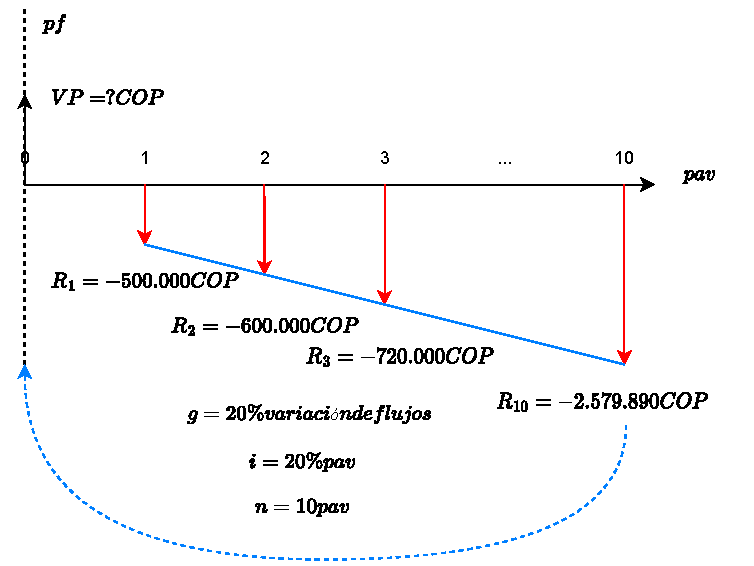
\includegraphics[trim=-5 -5 -5 -5 , scale=0.5]{6_Capitulo/img/ejemplos/7/Capitulo6Ejemplo7.pdf} }
		
		\\ \hline
		%%%%%%%%%%%%% FIN INSERCIÓN DE IMAGEN
		%%%%%FIN FLUJO DE CAJA
		
		%%%%% INICIO DECLARACIÓN FORMULAS
		%%%%%%%%%%% INICIO TITULO
		\rowcolor[HTML]{FFB183}
		\multicolumn{3}{|c|}{\cellcolor[HTML]{FFB183}\textbf{4. Declaración de fórmulas}}    \\ \hline
		%%%%%%%%%%% FIN TITULO
		%%%%%%%%%%% INICIO MATEMÁTICAS
		
		\multicolumn{3}{|c|}{$VP=(\frac{(R)(n)}{1+i}) \hspace{0.4 cm} \textit{Valor presente de un gradiente geometrico para i=g}$} \\ 
		\multicolumn{3}{|c|}{$R_n=(R_1(1+g)^{n-1}) \hspace{0.4 cm} \textit{Valor del flujo de un gradiente geométrico}$} \\ \hline
		
		%%%%%%%%%% FIN MATEMÁTICAS
		%%%%%% INICIO DESARROLLO MATEMÁTICO
		\rowcolor[HTML]{FFB183}
		%%%%%%%%%%INICIO TITULO
		\multicolumn{3}{|c|}{\cellcolor[HTML]{FFB183}\textbf{5. Desarrollo matemático}}       \\ \hline
		%%%%%%%%%% FIN TITULO
		%%%%%%%%%% INICIO MATEMÁTICAS
		
		\multicolumn{3}{|c|}{$VP=(\frac{( 500{.}000COP)(10)}{1+0,2}) \hspace{0.2 cm}\rightarrow \hspace{0.2 cm} VP=  4{.}166{.}667COP$} \\ \hline
		%%%%%%%%%% FIN MATEMÁTICAS
		%%%%%% FIN DESARROLLO MATEMÁTICO
		%%%%%% INICIO RESPUESTA
		\rowcolor[HTML]{FFB183}
		%%%%%%%%%%INICIO TITULO
		\multicolumn{3}{|c|}{\cellcolor[HTML]{FFB183}\textbf{6. Respuesta}}   \\ \hline
		%%%%%%%%%% FIN TITULO
		%%%%%%%%%% INICIO RESPUESTA MATEMÁTICA
		\multicolumn{3}{|c|}{${VP=  4{.}166{.}667 COP}$} 
		\\ \hline
		%%%%%%%%%% FIN MATEMÁTICAS
		%%%%%% FIN RESPUESTA
	\end{longtable}
	%Se crean dos lineas en blanco para que no quede el siguiente texto tan pegado
	%\newline \newline %USARLO SI CREES QUE ES NECESARIO
\end{center}
%%%%%%%%%%%%%%%%%%%%%%%%%%FIN EJERCICIO 7 %%%%%%%%%%%%%%%%%%%%%%%%%%%

	%%%%%%%%%%%%%%%%%%%%%%%%%%%%%%%%%%%%%%%%%%%%%%%%%%%%%%%%%%%%%%%%%%%%%%%%%%%%%%%%%%%%%%%%%%%%%%%%%%%%%%%%%%%%%%
	
	%COMENTADO
	\begin{comment}
	\textbf{Ejemplo 9}\\
	Hallar el valor de la cuota total que debe ser pagada al final del mes 12, para amortizar una deuda de  COP  3 millones con pago anticipado de interés y abonos mensuales constantes a capital, durante 4 años, con un interés del 2\% período mes anticipado.\\
	
	\textbf{Solución: }\\
	\textbf{a.}	Diagrama de flujo de caja
	\begin{center}
		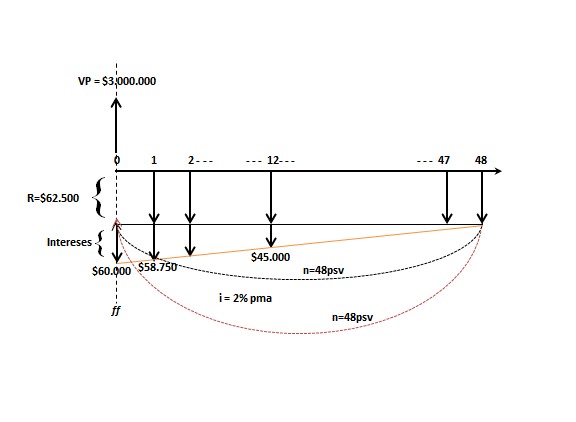
\includegraphics[height=10.00cm]{7_22}
	\end{center}
	\textbf{b.}	Declaración de variables:\\
	
	
	$I=F*i_{a} \hspace{35 pt} \textit{Monto de intereses periódicos anticipados}\\
		A=\frac{P}{n} \hspace{35 pt} \textit{Amortización igual a capital en n períodos}\\
		R=A+i$ \\
	
	
	\textbf{c.}	Declaración de fórmulas:
	\begin{align*}
		VP=\frac{R}{i}
	\end{align*}
	\textbf{d.} Desarrollo matemático:
	Se puede observar que entre el primer pago de intereses que se hace en el período cero (por ser anticipado) y el último pago de intereses (período 47) forma un gradiente lineal decreciente, mientras que el primer abono a capital se hace en el período 1 (por ser vencido).\\
	
	Como los intereses forman un gradiente lineal decreciente, necesitamos calcular el valor L de decrecimiento en la siguiente forma:\\
	
	Interés del período cero:
	\begin{align*}
		I= 3.000.000  COP  x0,02  =  60,000  COP
	\end{align*}
	Deuda al final del primer período:
	\begin{align*}
		I= 3.000 000  COP  - COP   62.500  =  2.937.500  COP
	\end{align*}
	Interés al final del primer período:
	\begin{align*}
		I= 2.937.500  COP  * 0,02  =  58.750  COP
	\end{align*}
	Variación del interés:
	\begin{align*}
		L=  1.250  COP
	\end{align*}
	Ahora, necesitamos calcular los intereses al final del período 12 que corresponden al pago número 13 del gradiente:\\
	
	\
	$R_{13}=R_{1}  + (n-1)L=  60.000  COP+ (13 -1)( -  1. 250  COP)=  45.000  COP$\\
	
	
	El pago que debe hacerse al final del período 12 será igual a la suma de la cuota de interés, más la cuota de abono a capital, esto es:\\
	
	
	$R_{13}=  45.000  COP  +    62.500  COP  =  107.500  COP  $\\
	
	
	Otra forma de resolver el problema anterior es calculando la deuda en el punto 12 y multiplicando por la tasa.\\
	
	\textbf{e.}	Respuesta:\\
	
	Como en total hay 48 pagos y ya se han hecho 12, faltan 36 pagos por hacer, esto es:\\
	
	
	F=36 pma x  62.500  COP  =  225.000  COP\\
	36 x   62.500  COP  =   2.250.000  COP\\
	
	
	Intereses:
	
	
	F= 2'250.000  COPx 0,02=  45.000  COP\\
	
	
	Valor total de la cuota:\\
	
	R=A+I\\
	
	
	R= 62.500  COP  +   45.000  COP  =  107.500  COP\\
	\end{comment}
	%\newpage
	\section{Amortización mediante gradientes escalonados}
	Los sistemas escalonados pueden ser lineales o geométricos y éstos a su vez pueden ser crecientes o decrecientes; mediante éste sistema se logra \textbf{COMBINAR} cuotas constantes con cuotas crecientes o decrecientes. Es decir que conservaremos constante la cuota de amortización, durante un tiempo determinado, al final del cual se incrementa o decrementa, según el caso.\\\\
	Examinaremos dos situaciones, la primera será la \textbf{FUSIÓN} de una cuota constante con un \textbf{gradiente geométrico}; la segunda será la \textbf{FUSIÓN} de una cuota constante con un \textbf{gradiente lineal}; en ambos casos será necesario construir dos gráficas. La primera corresponde a la forma como se van a pagar las cuotas y en la segunda cada serie de cuotas iguales será reemplazada por una sola cuota al final del período. A la primera gráfica se le denominará gradiente escalonado y la segunda gráfica corresponde al gradiente simple.\\\\
	%Las definiciones que hemos dado con anterioridad continuarán vigentes para la segunda gráfica, pero para la primera gráfica a todas las definiciones se les antepondrá el prefijo inter o el prefijo sub, por tanto.
	El valor de cada pago lo denominaremos intercuota o subcuota y lo representaremos por \textbf{“r”} (minúscula), el tiempo que transcurre entre dos intercuotas lo denominaremos interperíodo y la tasa correspondiente al interperíodo se denominará intertasa o subtasa. Además, el número de intercuotas que hay por cada cuota es constante y se representará por "m" e indicará el tamaño del escalón, además, la altura del escalón vendrá dada por la diferencia que hay entre dos intercuotas cualesquiera pero de escalones contiguos y la representaremos por "H".\\\\
	%%%%%%%%%%%%%%%%%%%%%%%%%%%%%%%%%%%%%%%%%%%%%%%%%%%%%%%%%%%%%%%%%%%%%%%%%%%%%%%%%%%%%%%%%%%%%%%%%%%%%%%%%%%%%%%%%%%%%%%%%%%%%%%%%%%%%EJERCICIO 8 %%%%%%%%%%%%%%%%%%%%%%%%%%%
	\newpage
\textbf{Ejemplo 8}\\
Supongamos que un inversionista desea adquirir la aceptación bancaria del ejemplo anterior, la cual figura con una tasa de registro del 30\% periódico 40 días vencido y con precio de registro $P_r =  97,65 COP$ pero él también sabe que para adquirirla deberá pagar una comisión a un corredor de bolsa lo cual hará variar el precio que él debe pagar y también la rentabilidad que él pueda obtener. Supongamos que la comisión que cobra un corredor por la compra es del 0,475\% periodo 40 días periodo vencido ¿Cuál es el precio del inversionista Pc =  ? COP , que incluye la comisión del comisionista vendedor, el precio de registro y la comisión de bolsa del comprador. El punto de referencia es el precio de registro $P_r$ ¿Cuál es la rentabilidad del inversionista $i_c =? \%?$ periódica 40 días vencido, o $j=? \hspace{0.5mm} nadv$
%\newpage %USAR SOLO SI EL SOLUCIÓN QUEDA SOLO Y ES NECESARIO BAJARLO A LA SIGUIENTE PAGINA

\textbf{Solución.}
%La tabla ira centrada
\begin{center}
 \renewcommand{\arraystretch}{1.5}% Margenes de las celdas
 %Creación de la cuadricula de 3 columnas
 \begin{longtable}[H]{|p{0.5\linewidth}|p{0.5\linewidth}|}
  %Creamos una linea horizontal
  \hline
  %Definimos el color de la primera fila
  \rowcolor[HTML]{FFB183}
  %%%%% INICIO ASIGNACIÓN FECHA FOCAL %%%%%%%
  %%%%%%%%%% INICIO TITULO
  %Lo que se hace aquí es mezclar las 3 columnas en una sola
  \multicolumn{2}{|c|}{\cellcolor[HTML]{FFB183}\textbf{1. Asignación período focal}}                  \\ \hline
  %%%%%%%%%% FIN TITULO
  %%%%% INICIO DECLARACIÓN DE VARIABLES %%%%%%%
  \multicolumn{2}{|c|}{$pf = 40 \textit{ pdv}$}                                                     \\ \hline
  %%%%%%%%%% INICIO TITULO
  %Lo que se hace aquí es mezclar las 3 columnas en una sola
  \multicolumn{2}{|c|}{\cellcolor[HTML]{FFB183}\textbf{2. Declaración de variables}}                \\ \hline
  %%%%%%%%%% FIN TITULO
  %%%%%%%%%% INICIO DE MATEMÁTICAS
  %Cada & hace referencia al paso de la siguiente columna
  $i_c = 30\% -0,475\% = 29,525\% \hspace{1mm} p40dv$ & $P_R=?$                                     \\
  $P_c =  ? COP$                                         &                                             \\
  $n= \frac{40}{365} \hspace{1mm} p(40das) $          &                                             \\ \hline
  %%%%%%%%%% FIN DE MATEMÁTICAS
  %%%%% FIN DECLARACIÓN DE VARIABLES

  \rowcolor[HTML]{FFB183}
  \multicolumn{2}{|c|}{\cellcolor[HTML]{FFB183}\textbf{3. Diagrama de flujo de caja}}               \\ \hline
  \multicolumn{2}{|c|}{ 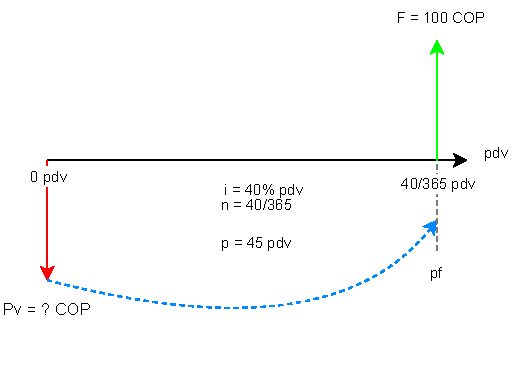
\includegraphics[trim=-78 0 -78 0]{3_Capitulo/img/ejemplos/8/capitulo3ejercicio8.pdf} }  \\ \hline
  %%%%% INICIO FLUJO DE CAJA
  \rowcolor[HTML]{FFB183}
  \multicolumn{2}{|c|}{\cellcolor[HTML]{FFB183}\textbf{4. DECLARACIÓN de formulas}}                 \\ \hline
  %Mezclamos 3 columnas y pondremos el dibujo
  %%%%%%%%%%%%% INSERCIÓN DE LA IMAGEN
  %Deberán descargar las imágenes respectivas del drive y pegarlas en la carpeta
  %n_capitulo/img/ejemplos/1/capitulo1ejemplo1.pdf  (el /1/ es el numero del ejemplo)
  \multicolumn{2}{|c|}{ $P = F(1 + i)^n $ Valor presente }                                          \\ \hline
  %%%%%%%%%%%%% FIN INSERCIÓN DE IMAGEN
  %%%%%FIN FLUJO DE CAJA


  %%%%%% INICIO DESARROLLO MATEMÁTICO
  \rowcolor[HTML]{FFB183}
  %%%%%%%%%%INICIO TITULO
  \multicolumn{2}{|c|}{\cellcolor[HTML]{FFB183}\textbf{5. Desarrollo matemático}}                   \\ \hline
  %%%%%%%%%% FIN TITULO
  %%%%%%%%%% INICIO MATEMÁTICAS
  \multicolumn{2}{|C{\linewidth}|}{
  $P_c =  100 COP(1 + 0,29525)\frac{40}{365} = 97,204 COP$ Ecuación de valor

  $P_R = 0,972047( 5{.}000{.}000 COP) =  4{.}860{.}245 COP$

  $P_c - P_R =  4{.}860{.}235 COP -  4{.}858{.}285 COP = 1{.}950 COP$
  }                                                                                                 \\ \hline

  %%%%%%%%%% FIN MATEMÁTICAS
  %%%%%% FIN DESARROLLO MATEMÁTICO
  %%%%%% INICIO RESPUESTA
  \rowcolor[HTML]{FFB183}
  %%%%%%%%%%INICIO TITULO
  \multicolumn{2}{|c|}{\cellcolor[HTML]{FFB183}\textbf{6. Respuesta}}                               \\ \hline
  %%%%%%%%%% FIN TITULO
  %%%%%%%%%% INICIO RESPUESTA MATEMÁTICA
  \multicolumn{2}{|C{\textwidth}|}{
  $P_R =  4{.}860{.}245 COP$
  }                                                                                                 \\ \hline


  %%%%%%%%%% FIN MATEMÁTICAS
  %%%%%% FIN RESPUESTA
 \end{longtable}
 %Se crean dos lineas en blanco para que no quede el siguiente texto tan pegado
 %\newline \newline %USARLO SI CREES QUE ES NECESARIO
\end{center}
	%%%%%%%%%%%%%%%%%%%%%%%%%%FIN EJERCICIO 8 %%%%%%%%%%%%%%%%%%%%%%%%%%%%%%%%%%%%%%%%%%%%%%%%%%%%%%%%%%%%%%%%%%%%%%%%%%%%%%%%%%%%%%%%%%%%%%%%%%%%%%%
	
	\begin{comment}
	\textbf{Ejemplo 11}\\
	Elaborar una tabla para amortizar la suma de 600.000 COP en 4 pagos anuales e iguales, pero en valor constante, suponga una tasa de interés del 8\% período trimestre vencido y que:\\
	
	a)	la corrección monetaria permanecerá constante en el 22\% durante los 4 años.\\
	b)	la corrección monetaria es del 22\% en los 2 primeros años, del 24\% para el tercer año y del 27\% para el cuarto año.\\
	
	\textbf{Solución a:}\\
	\textbf{a.}	Diagrama de flujo de caja:
	\begin{center}
		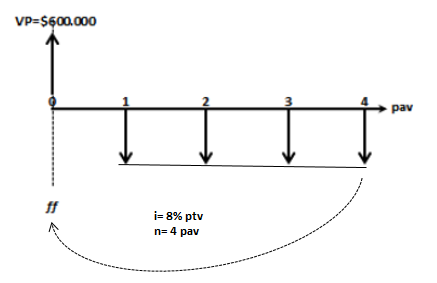
\includegraphics[height=5.0cm]{7_29}
	\end{center}
	
	\textbf{b.}	Declaración de variables:\\
	
	VP= COP   600.000\\
	i\equiv 8 \%  $\ \ ptv\\
	n=4 \ \ pav\\
	R=  COP  ?\\
	
	\textbf{c.}	Declaración de fórmulas:\\
	
	$VP=R \frac{1-(1+i)^{-n}}{i} \hspace{35pt}\textit{Valor presente serie uniforme vencida}$\\
	
	\textbf{d.}	Desarrollo matemático:\\
	Primero calculamos el valor de la cuota haciendo caso omiso de la corrección monetaria\\
	
	
	$ COP   600.000= R \frac{1-(1+0,08)^{-4}}{0,08}$ \\
	
	R= COP   181.152,48\\
	
	El valor de  COP  181.152,48 corresponde al valor de las cuotas pero en pesos de hoy, sin embargo, cuando se vaya a pagar la primera cuota este valor se debe incrementar debido a la corrección monetaria y será:\\
	
	Primera cuota:	 $ COP  181.152,48 x (1 +0,22)   = COP  221.006,03$\\
	Segunda cuota:	 $ COP  181.152,48 x (1 +0.22)^{2}= COP  269 627.35$\\
	Tercera cuota:	 $ COP  181.152,48 x (1 +0.22)^{3}= COP  328.945,37$ \\
	Cuarta cuota:	 $ COP  181.152,48 x (1 +0,22)^{4}= COP  401.313,35$ \\
	
	Así como hemos corregido el valor de las cuotas tenemos que corregir los saldos de la deuda y para ello será necesario incluir en la tabla una nueva columna que denominaremos ''capital insoluto ajustado'', donde colocaremos, los saldos de la deuda ajustados con la corrección monetaria al final de cada período.\\
	
	\textbf{e.	}Respuesta:\\
	El saldo insoluto ajustado del período cero se obtiene al aplicarle la corrección monetaria al saldo insoluto del período cero, esto es:
	\begin{align*}
		 COP  600.000 x (1+0,22)= COP  732.000
	\end{align*}
	Sobre los  COP  732.000 se calculan los intereses así:
	\begin{align*}
		 COP  732.000 x 0,08= COP  58.560,00
	\end{align*}
	Si al saldo ajustado del período cero se le resta la amortización se tendrá el saldo (sin ajustar) al comienzo del primer período así:
	\begin{align*}
		 COP  732.000- COP  162.446,03= COP  569.553,97
	\end{align*}
	Este saldo se deberá ajustar para saber cuál es la deuda al final del mismo período, entonces se tendrá:
	\begin{align*}
		 COP  569.553,97 x (1 +0,22)= COP  694.855,84
	\end{align*}
	Al saldo insoluto ajustado del período 1 se le aplica la tasa de interés para obtener los intereses así:
	\begin{align*}
		 COP  694.855,84 x 0,08 = COP  55.588,47
	\end{align*}
	El resto de la tabla continúa en forma similar:
	
	\begin{spacing}{1.1}
		\begin{center}
			\begin{tabular}{|p{1cm}|p{3cm}|p{2cm}|p{2cm}|p{2cm}||p{3cm}|}
				\hline
				\rowcolor{white!50}
				\textbf{PER\ (1)} & \textbf{SALDO AJUSTADO } & \textbf{SALDO (3)=(3)-(6)} & \textbf{INTERESES  (4)=(3)*(i)} & \textbf{PAGO\ (5)= COP  R- COP  L } & \textbf{AMORTIZACIÓN  (6)=(5)-(4)} \\ \hline
				
				0                 &  COP  600.000,00             &  COP  732.000,00               &  COP  0,00                          &  COP  0,00                      &  COP   0,00                            \\ \hline
				1                 &  COP  569.553,97             &  COP   694.855,84              &  COP  58.560,00                     &  COP  221.006,03                &  COP   214.038,88                      \\ \hline
				2                 &  COP  480.816,96             &  COP   371.586,45              &  COP  46.927,74                     &  COP  328.945,37                &  COP  282.017,64                       \\ \hline
				3                 &  COP  304.779,06             &  COP  371.586,45               &  COP  46.927,74                     &  COP  328.945,37                &  COP  282.017,64                       \\ \hline
				4                 &  COP  0,00                   &  COP  0,00                     &  COP  29.726,90                     &  COP  401.313,35                &  COP  371.586,45                       \\ \hline
			\end{tabular}
		\end{center}
	\end{spacing}
	
	
	\textbf{Solución b:}\\
	Igual que en la parte a) calculamos el valor de la cuota haciendo caso omiso de la corrección monetaria y el valor de ésta, resulta ser en pesos de hoy,  COP  181 152.48, y el valor de lo que se debe pagar anualmente, será:\\
	
	Primera cuota:	 $ COP  181.152,48 x (1 +0,22)   = COP  221.006,03$\\
	Segunda cuota:	 $ COP  181.152,48 x (1 +0,22)^{2}= COP  269.627,35$\\
	Tercera cuota:	 $ COP  181.152,48 x (1 +0,22)^{2}  x (1 +0,24)= COP  334.337,91 $\\
	Cuarta cuota:	 $ COP  181.152,48 x (1 +0,22)^{2}  x (1+0,24)X (1+0,27)= COP  424.609,15$\\
	
	Al elaborar la tabla debe tenerse en cuenta que el factor de ajuste del capital insoluto del período 2 será: (1 +0,24) y el factor de ajuste del capital insoluto del período 3 será (1 +0,27) y la tabla quedará así:
	
	\begin{spacing}{1.1}
		\begin{center}
			\begin{tabular}{|p{1cm}|p{2cm}|p{3cm}|p{2cm}|p{2cm}||p{3cm}|}
				\hline
				\rowcolor{white!50}
				\textbf{PER\ (1)} & \textbf{SALDO (2)=(2)-(6)} & \textbf{SALDO AJUSTADO } & \textbf{INTERESES  (4)=(2)(i)} & \textbf{PAGO\ (5)= COP  R- COP  L } & \textbf{AMORTIZACIÓN  (2)=(5)-(4)} \\ \hline
				
				0                 &  COP  600.000,00               &  COP  732.000,00             &  COP  0,00                          &  COP  0,00                      &  COP   0,00                            \\ \hline
				1                 &  COP  569.553,97               &  COP   694.855,84            &  COP  58.560,00                     &  COP  221.006,03                &  COP   162.446,03                      \\ \hline
				2                 &  COP  480.816,96               &  COP   596.213,03            &  COP  55.588,47                     &  COP  269.627,35                &  COP  214.038,88                       \\ \hline
				3                 &  COP  309.572,16               &  COP  393.156,64             &  COP  47.697,04                     &  COP  334.337,91                &  COP  286.640,87                       \\ \hline
				4                 &  COP  0,00                     &  COP  0,00                   &  COP  31.452,51                     &  COP  424.609,51                &  COP  424.609,15                       \\ \hline
			\end{tabular}
		\end{center}
	\end{spacing}
	\end{comment}
	
	%\textbf{Ejemplo 12}\\
	
	
	%%%%%%%%%%%%%%%%%%%%%%%%%%%%%%%%%%%%%%%%%%%%%%%%%%%%%%%%%%%%%%%%%%%%%%%%%%%%%%%%%%%%%%%%%%%%%%%%%%%%%%%%%%%%%%%%%%%%%%%%%%%%%%%%%%%%%EJERCICIO 9 %%%%%%%%%%%%%%%%%%%%%%%%%%%
	\textbf{Ejemplo 9}\\
Elaborar una tabla para amortizar la suma de  100.000 COP en 4 pagos, suponiendo una tasa del 8\% periódica anual vencida:
\begin{itemize}
	\item a. Crecimiento geométrico periódico de 10\% de los flujos
	\item b. Decrecimiento geométrico periódico de 10\% de los flujos
\end{itemize}
	
	%%%%%%%%%%%%%%%%%%% EJERCICIO 9a %%%%%%

%\newpage %USAR SOLO SI EL SOLUCIÓN QUEDA SOLO Y ES NECESARIO BAJARLO A LA SIGUIENTE PAGINA
\textbf{Solución a.}\\
%La tabla ira centrada
\begin{center}
	\renewcommand{\arraystretch}{1.6}% Margenes de las celdas
	%Creación de la cuadricula de 3 columnas
	\begin{longtable}[H]{|c|c|c|}
		%Creamos una linea horizontal
		\hline
		%Definimos el color de la primera fila
		\rowcolor[HTML]{FFB183}
		%%%%% INICIO ASIGNACIÓN FECHA FOCAL %%%%%%%
		%%%%%%%%%% INICIO TITULO
		%Lo que se hace aquí es mezclar las 3 columnas en una sola
		\multicolumn{3}{|c|}{\cellcolor[HTML]{FFB183}\textbf{1. Asignación período focal}}  \\ \hline
		\multicolumn{3}{|c|}{$pf = \textit{0 pav}$}   \\\hline
		%%%%%%%%%% FIN TITULO
		%%%%% INICIO DECLARACIÓN DE VARIABLES %%%%%%%
		%%%%%%%%%% INICIO TITULO
		%Lo que se hace aquí es mezclar las 3 columnas en una sola
		\multicolumn{3}{|c|}{\cellcolor[HTML]{FFB183}\textbf{2. Declaración de variables}}   \\ \hline
		%%%%%%%%%% FIN TITULO
		%%%%%%%%%% INICIO DE MATEMÁTICAS
		%Cada & hace referencia al paso de la siguiente columna
		\multicolumn{2}{|c|}{$\hspace{2 cm}R=  100{.}000 COP \hspace{2 cm}$} & $i=8\% \textit{ pav}$ \\
		\multicolumn{2}{|c|}{$\hspace{2 cm}n=4  \textit{ pav} \hspace{2 cm}$} & $g=10\% \textit{creicente geometrico periódico con } g \neq i$ \\ \hline	
		
		
		%%%%%%%%%% FIN DE MATEMÁTICAS
		%%%%% FIN DECLARACIÓN DE VARIABLES
		
		%%%%% INICIO FLUJO DE CAJA
		\rowcolor[HTML]{FFB183}
		\multicolumn{3}{|c|}{\cellcolor[HTML]{FFB183}\textbf{3. Diagrama de flujo de caja}} \\ \hline
		%Mezclamos 3 columnas y pondremos el dibujo
		%%%%%%%%%%%%% INSERCIÓN DE LA IMAGEN
		%Deberán descargar las imágenes respectivas del drive y pegarlas en la carpeta
		%n_capitulo/img/ejemplos/1/capitulo1ejemplo1.pdf  (el /1/ es el numero del ejemplo)
		\multicolumn{3}{|c|}{ 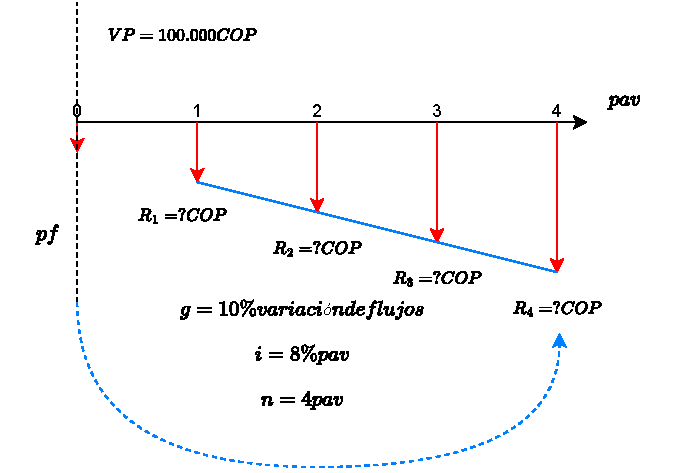
\includegraphics[trim=-5 -5 -5 -5 , scale=0.6]{6_Capitulo/img/ejemplos/9/Capitulo6Ejemplo9a.pdf} }
		\\ \hline
		%%%%%%%%%%%%% FIN INSERCIÓN DE IMAGEN
		%%%%%FIN FLUJO DE CAJA
		
		%%%%% INICIO DECLARACIÓN FORMULAS
		%%%%%%%%%%% INICIO TITULO
		\rowcolor[HTML]{FFB183}
		\multicolumn{3}{|c|}{\cellcolor[HTML]{FFB183}\textbf{4. Declaración de fórmulas}}    \\ \hline
		%%%%%%%%%%% FIN TITULO
		%%%%%%%%%%% INICIO MATEMÁTICAS
		\multicolumn{3}{|c|}{$VP=(\frac{(R)[(1+g)^{n}(1+i)^{-n}-1]}{g-i}) \hspace{0.4 cm} \textit{Valor presente de un gradiente aritmético }$} \\  
		\multicolumn{3}{|c|}{$R_n=(R_1(1+g)^{n-1}) \hspace{0.4 cm} \textit{Valor del flujo de n gradiente geométrico}$} \\ \hline
		
		%%%%%%%%%% FIN MATEMÁTICAS
		%%%%%% INICIO DESARROLLO MATEMÁTICO
		\rowcolor[HTML]{FFB183}
		%%%%%%%%%%INICIO TITULO
		\multicolumn{3}{|c|}{\cellcolor[HTML]{FFB183}\textbf{5. Desarrollo matemático}}       \\ \hline
		%%%%%%%%%% FIN TITULO
		%%%%%%%%%% INICIO MATEMÁTICAS
		\multicolumn{3}{|c|}{$100{.}000COP=(\frac{(R_1)[(1+0.1)^{4}(1+0.08)^{-4}-1]}{0.1-0.08})$} \\
		\multicolumn{3}{|c|}{$R_1=  26{.}261.47 COP$}\\ 
		\multicolumn{3}{|c|}{$R_2=  26{.}261.47(1+0.1) COP=   28{.}887.61COP$}\\
		\multicolumn{3}{|c|}{$R_3=  26{.}261.47(1+0.1)^2 COP=   31{.}776.38COP$}\\
		\multicolumn{3}{|c|}{$R_4=  26{.}261.47(1+0.1)^3 COP=   34{.}954.01COP$}\\ \hline
		%%%%%%%%%% FIN MATEMÁTICAS
		%%%%%% FIN DESARROLLO MATEMÁTICO
		%%%%%% INICIO RESPUESTA
		\rowcolor[HTML]{FFB183}
		%%%%%%%%%%INICIO TITULO
		\multicolumn{3}{|c|}{\cellcolor[HTML]{FFB183}\textbf{6. Respuesta}}   \\ \hline
		%%%%%%%%%% FIN TITULO
		%%%%%%%%%% INICIO RESPUESTA MATEMÁTICA
		\multicolumn{3}{|c|}{$R_1=  26{.}261COP$}\\ 
		\multicolumn{3}{|c|}{$R_2=  28{.}888 COP$}\\
		\multicolumn{3}{|c|}{$R_3=  31{.}776 COP$}\\
		\multicolumn{3}{|c|}{$R_4=  34{.}954 COP$}\\ \hline
		%%%%%%%%%% FIN MATEMÁTICAS
		%%%%%% FIN RESPUESTA
	\end{longtable}
	%Se crean dos lineas en blanco para que no quede el siguiente texto tan pegado
	%\newline \newline %USARLO SI CREES QUE ES NECESARIO
\end{center}

%%%%%%%%%%%%%%%%%%%%%%%%%%FIN EJERCICIO 9a %%%%%%%%%%%%%%%%%%%%%%%%%%%
	      \begin{spacing}{1.1}
	      	\begin{center}
	      		\begin{tabular}{|p{1cm}|p{2cm}|p{2.1cm}|p{2cm}|p{3cm}|}
	      			\hline
	      			\rowcolor{white!50}
	      			\textbf{n\ } & \textbf{Saldo Deuda COP} & \textbf{Intereses  COP} & \textbf{Pago COP} & \textbf{Amortización COP } \\ \hline
	      			
	      			0            &   100.000         &      -       &   -    &        -      \\ \hline
	      			1            &   81.739             &   8.000           &   26.261       &   18.261            \\ \hline
	      			2            &   59.390             &   6539,13              &   28.888       &   22.348,88              \\ \hline
	      			3            &   32.365.21            &   4751,2             &   31.776      &   27.024,79              \\ \hline
	      			4            &   0            &   2589,22            &   34.954       &   32.365,21              \\ \hline
	      		\end{tabular}
	      	\end{center}
	      \end{spacing}

	%%%%%%%%%%%%%%%%%%% EJERCICIO 9b %%%%%%

%\newpage %USAR SOLO SI EL SOLUCIÓN QUEDA SOLO Y ES NECESARIO BAJARLO A LA SIGUIENTE PAGINA
\textbf{Solución b.}\\
%La tabla ira centrada
\begin{center}
	\renewcommand{\arraystretch}{1.6}% Margenes de las celdas
	%Creación de la cuadricula de 3 columnas
	\begin{longtable}[H]{|c|c|c|}
		%Creamos una linea horizontal
		\hline
		%Definimos el color de la primera fila
		\rowcolor[HTML]{FFB183}
		%%%%% INICIO ASIGNACIÓN FECHA FOCAL %%%%%%%
		%%%%%%%%%% INICIO TITULO
		%Lo que se hace aquí es mezclar las 3 columnas en una sola
		\multicolumn{3}{|c|}{\cellcolor[HTML]{FFB183}\textbf{1. Asignación período focal}}  \\ \hline
		\multicolumn{3}{|c|}{$pf = \textit{0 pav}$}   \\\hline
		%%%%%%%%%% FIN TITULO
		%%%%% INICIO DECLARACIÓN DE VARIABLES %%%%%%%
		%%%%%%%%%% INICIO TITULO
		%Lo que se hace aquí es mezclar las 3 columnas en una sola
		\multicolumn{3}{|c|}{\cellcolor[HTML]{FFB183}\textbf{2. Declaración de variables}}   \\ \hline
		%%%%%%%%%% FIN TITULO
		%%%%%%%%%% INICIO DE MATEMÁTICAS
		%Cada & hace referencia al paso de la siguiente columna
		\multicolumn{2}{|c|}{$\hspace{2 cm}VP= 100{.}000 COP \hspace{2 cm}$} & $i=8\% \textit{ pav}$ \\
		\multicolumn{2}{|c|}{$\hspace{2 cm}n=4  \textit{ pav} \hspace{2 cm}$} & $g=-10\% \textit{decreicente con } g \neq i$ \\ \hline	
		
		%%%%%%%%%% FIN DE MATEMÁTICAS
		%%%%% FIN DECLARACIÓN DE VARIABLES
		
		%%%%% INICIO FLUJO DE CAJA
		\rowcolor[HTML]{FFB183}
		\multicolumn{3}{|c|}{\cellcolor[HTML]{FFB183}\textbf{3. Diagrama de flujo de caja}} \\ \hline
		%Mezclamos 3 columnas y pondremos el dibujo
		%%%%%%%%%%%%% INSERCIÓN DE LA IMAGEN
		%Deberán descargar las imágenes respectivas del drive y pegarlas en la carpeta
		%n_capitulo/img/ejemplos/1/capitulo1ejemplo1.pdf  (el /1/ es el numero del ejemplo)
		\multicolumn{3}{|c|}{ 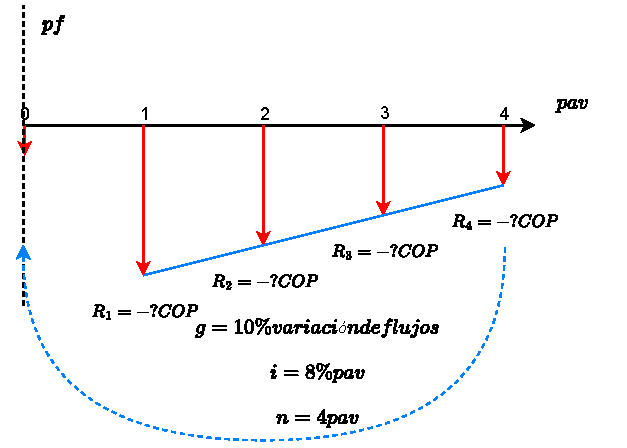
\includegraphics[trim=-5 -5 -5 -5 , scale=0.6]{6_Capitulo/img/ejemplos/9/Capitulo6Ejemplo9b.pdf} }
		\\ \hline
		%%%%%%%%%%%%% FIN INSERCIÓN DE IMAGEN
		%%%%%FIN FLUJO DE CAJA
		
		%%%%% INICIO DECLARACIÓN FORMULAS
		%%%%%%%%%%% INICIO TITULO
		\rowcolor[HTML]{FFB183}
		\multicolumn{3}{|c|}{\cellcolor[HTML]{FFB183}\textbf{4. Declaración de fórmulas}}    \\ \hline
		%%%%%%%%%%% FIN TITULO
		%%%%%%%%%%% INICIO MATEMÁTICAS
		\multicolumn{3}{|c|}{$VP=(\frac{(R)[(1+g)^{n}(1+i)^{-n}-1]}{g-i}) \hspace{0.4 cm} \textit{Valor presente de un gradiente aritmético }$} \\  
		\multicolumn{3}{|c|}{$R_n=(R_1(1+g)^{n-1}) \hspace{0.4 cm} \textit{Valor del flujo de n gradiente geométrico}$} \\ \hline
		
		%%%%%%%%%% FIN MATEMÁTICAS
		%%%%%% INICIO DESARROLLO MATEMÁTICO
		\rowcolor[HTML]{FFB183}
		%%%%%%%%%%INICIO TITULO
		\multicolumn{3}{|c|}{\cellcolor[HTML]{FFB183}\textbf{5. Desarrollo matemático}}       \\ \hline
		%%%%%%%%%% FIN TITULO
		%%%%%%%%%% INICIO MATEMÁTICAS
		\multicolumn{3}{|c|}{$  100{.}000COP=(\frac{(R_1)[(1-0.1)^{4}(1+0.08)^{-4}-1]}{-0.1-0.08})$} \\
		\multicolumn{3}{|c|}{$R_1=  34{.}766 COP$}\\ 
		\multicolumn{3}{|c|}{$R_2=  34{.}766.02COP(1-0.1)  =   31{.}289.42COP$}\\
		\multicolumn{3}{|c|}{$R_3=  34{.}766.02COP(1-0.1)^2 =   28{.}160.48COP$}\\
		\multicolumn{3}{|c|}{$R_4=  34{.}766.02COP(1-0.1)^3 =   25{.}344.43COP$}\\ \hline
		%%%%%%%%%% FIN MATEMÁTICAS
		%%%%%% FIN DESARROLLO MATEMÁTICO
		%%%%%% INICIO RESPUESTA
		\rowcolor[HTML]{FFB183}
		%%%%%%%%%%INICIO TITULO
		\multicolumn{3}{|c|}{\cellcolor[HTML]{FFB183}\textbf{6. Respuesta}}   \\ \hline
		%%%%%%%%%% FIN TITULO
		%%%%%%%%%% INICIO RESPUESTA MATEMÁTICA
		\multicolumn{3}{|c|}{$R_1=  34{.}766COP$}\\ 
		\multicolumn{3}{|c|}{$R_2=  31{.}289COP$}\\
		\multicolumn{3}{|c|}{$R_3=  28{.}160COP$}\\
		\multicolumn{3}{|c|}{$R_4=  25{.}344COP$}\\ \hline
		%%%%%%%%%% FIN MATEMÁTICAS
		%%%%%% FIN RESPUESTA
	\end{longtable}
	%Se crean dos lineas en blanco para que no quede el siguiente texto tan pegado
	%\newline \newline %USARLO SI CREES QUE ES NECESARIO
\end{center}

%%%%%%%%%%%%%%%%%%%%%%%%%%FIN EJERCICIO 9b %%%%%%%%%%%%%%%%%%%%%%%%%%%
	      
	      \begin{spacing}{1.1}
		      \begin{center}
			      \begin{tabular}{|p{1cm}|p{2cm}|p{2.1cm}|p{2cm}|p{2.5cm}|}
				      \hline
				      \rowcolor{white!50}
				      \textbf{n\ } & \textbf{Saldo Deuda COP} & \textbf{Intereses COP } & \textbf{Pago COP } & \textbf{Amortización COP} \\ \hline
				      
				      0            &   100.000         & -    & -  & -    \\ \hline
				      1            &   73.234           &   8.000          &   34.766      &   26.766             \\ \hline
				      2            &   47.803,72           &   5858,72             &   31.289      &   25.430,28             \\ \hline
				      3            &   23.468,01           &   3824,29             &   28.160      &   24.335,7            \\ \hline
				      4            &   0               &   1877,44             &   25.344,73      &   23.468,01             \\ \hline
			      \end{tabular}
		      \end{center}
	      \end{spacing}

	%%%%%%%%%%%%%%%%%%%%%%%%%%FIN EJERCICIO 9 %%%%%%%%%%%%%%%%%%%%%%%%%%%
	
	
	%%%%%%%%%%%%%%%%%%%%%%%%%%EJERCICIO 10 %%%%%%%%%%%%%%%%%%%%%%%%%%%
    %%%%%%%%%%%%%%%%%%%%%%%%%%EJERCICIO 10 %%%%%%%%%%%%%%%%%%%%%%%%%%%
 \textbf{Ejemplo 10}\\
	Resolver el problema anterior, suponiendo que el gradiente es escalonado con pagos semestrales.\\		
	
	\textbf{Solución 10}\\
	%La tabla ira centrada
	\begin{center}
		\renewcommand{\arraystretch}{1.5}% Margenes de las celdas
		%Creación de la cuadricula de 3 columnas
		\begin{longtable}[H]{|p{0.5\linewidth}|p{0.5\linewidth}|}
			%Creamos una linea horizontal
			\hline
			%Definimos el color de la primera fila
			\rowcolor[HTML]{FFB183}
			%%%%% INICIO ASIGNACIÓN período FOCAL %%%%%%%
			%%%%%%%%%% INICIO TITULO
			%Lo que se hace aquí es mezclar las 3 columnas en una sola
			\multicolumn{2}{|c|}{\cellcolor[HTML]{FFB183}\textbf{1. Asignación período focal}}   \\ \hline
			%%%%%%%%%% FIN TITULO
			%%%%% INICIO DECLARACIÓN DE VARIABLES %%%%%%%
			\multicolumn{2}{|c|}{$pf = 0 \textit{ psv}$}\\ \hline
			%%%%%%%%%% INICIO TITULO
			%Lo que se hace aquí es mezclar las 3 columnas en una sola
			\multicolumn{2}{|c|}{\cellcolor[HTML]{FFB183}\textbf{2. Declaración de variables}}   \\ \hline
			%%%%%%%%%% FIN TITULO
			%%%%%%%%%% INICIO DE MATEMÁTICAS
			%Cada & hace referencia al paso de la siguiente columna
			$VP = 500.000 \ COP $  				& $ n_{2}= 2 \hspace{1mm} psv $  \\
			$i \equiv  10\% \hspace{1mm} pav$      	& $ n_{3}= 3 \hspace{1mm} psv $ \\
			$ n = 2 \hspace{1mm} psv $          & $ n_{5}= 5 \hspace{1mm} psv $\\ 
			$ n_{1}= 1 \hspace{1mm} psv $       & $ n_{6}= 6 \hspace{1mm} psv $ \\ 
			$ $      						    & $ i \equiv  ? \% psv $ \\ \hline
			%%%%%%%%%% FIN DE MATEMÁTICAS
			%%%%% FIN DECLARACIÓN DE VARIABLES
			
			\rowcolor[HTML]{FFB183}
			\multicolumn{2}{|c|}{\cellcolor[HTML]{FFB183}\textbf{3. Diagrama de flujo de caja}} \\ \hline
			\multicolumn{2}{|c|}{ 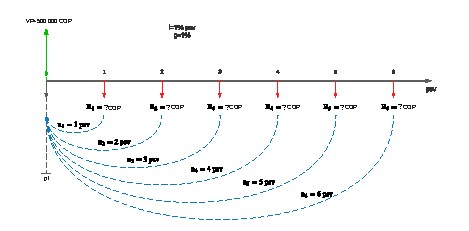
\includegraphics[trim=-78 -5 -78 -5]{7_Capitulo/img/ejemplos/10/10_1.pdf} }   \\ \hline
			%%%%% INICIO FLUJO DE CAJA
			\rowcolor[HTML]{FFB183}
			\multicolumn{2}{|c|}{\cellcolor[HTML]{FFB183}\textbf{4. Declaración de fórmulas}} \\ \hline
			%%%%%%%%%%%%% FIN INSERCIÓN DE IMAGEN
			%%%%%FIN FLUJO DE CAJA
			
			\multicolumn{2}{|c|}{ $(1+i_1)^{m_1} = (1+i_2)^{m_2} $ Equivalencia de tasas}   \\  
			\multicolumn{2}{|c|}{ $VF = R\frac{(1+i)^{n} -1 }{i} $ Valor presente serie uniforme}   \\  \hline
			
			%%%%%% INICIO DESARROLLO MATEMÁTICO
			\rowcolor[HTML]{FFB183}
			%%%%%%%%%%INICIO TITULO
			\multicolumn{2}{|c|}{\cellcolor[HTML]{FFB183}\textbf{5. Desarrollo matemático}}       \\ \hline
			%%%%%%%%%% FIN TITULO
			%%%%%%%%%% INICIO MATEMÁTICAS
			\multicolumn{2}{|c|}{  $(1+ 0,24)^{1} = (1+i)^{2} $}   \\ 
			\multicolumn{2}{|c|}{ $  i = 11,3552873\% \hspace{1mm} psv $}   \\  \hline
			
			%%%%%%%%%% FIN MATEMÁTICAS
			%%%%%% FIN DESARROLLO MATEMÁTICO
			%%%%%% INICIO RESPUESTA
			\rowcolor[HTML]{FFB183}
			%%%%%%%%%%INICIO TITULO
			\multicolumn{2}{|c|}{\cellcolor[HTML]{FFB183}\textbf{6. Respuesta}}   \\ \hline
			%%%%%%%%%% FIN TITULO
			%%%%%%%%%% INICIO RESPUESTA MATEMÁTICA
			\multicolumn{2}{|c|}{ 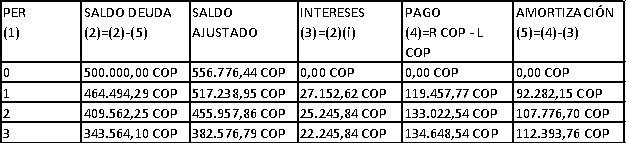
\includegraphics[trim=-78 -5 -78 -5]{7_Capitulo/img/ejemplos/10/10_2.pdf} }   \\ \hline
			%\multicolumn{2}{|C{\textwidth}|}{
			%	$R_{58} = 72.478,16 \ COP (1 + 0,02)^{57} = \ COP 224.087,15 $ 
			%}  \\ \hline
			
			
			%%%%%%%%%% FIN MATEMÁTICAS
			%%%%%% FIN RESPUESTA
		\end{longtable}
		%Se crean dos lineas en blanco para que no quede el siguiente texto tan pegado
		%\newline \newline %USARLO SI CREES QUE ES NECESARIO
	\end{center}
 %%%%%%%%%%%%%%%%%%%%%%%%%%FIN EJERCICIO 10 %%%%%%%%%%%%%%%%%%%%%%%%%%%
	%%%%%%%%%%%%%%%%%%%%%%%%%%FIN EJERCICIO 10 %%%%%%%%%%%%%%%%%%%%%%%%%%%
	
	
	\section{Capitalización diferida (*)}
	Se entiende por capitalización diferida a la capitalización que tiene uno o varios períodos en los cuales no se efectúan depósitos, pero el capital ahorrado si gana intereses. Es obvio que estos períodos se encontrarán entre la fecha del último depósito y la fecha de retiro del capital. \\
	
	
	%\textbf{Ejemplo 17}\\
	
	%%%%%%%%%%%%%%%%%%%%%%%%%%EJERCICIO 11 %%%%%%%%%%%%%%%%%%%%%%%%%%%%%%%%%%%%%%%%%%%%%%%%%%%%%%
	\textbf{Ejemplo 11}\\
Hallar el valor presente de 15 pagos que decrecen
linealmente en 400 COP, si el primer pago es de 5.000 COP y la tasa efectiva es del 4\% período año
vencido..\\ \\
%\newpage %USAR SOLO SI EL SOLUCIÓN QUEDA SOLO Y ES NECESARIO BAJARLO A LA SIGUIENTE PAGINA
\textbf{Solución.}\\
%La tabla ira centrada
\begin{center}
 \renewcommand{\arraystretch}{1.5}% Margenes de las celdas
 %Creación de la cuadricula de 3 columnas
 \begin{longtable}[H]{|p{0.5\linewidth}|p{0.5\linewidth}|}
  \hline
  \multicolumn{2}{|c|}{\cellcolor[HTML]{FFB183}\textbf{1. Declaración de variables}}                                                                                                                 \\ \hline
  $R =  5.400 COP$                                                                                & $L = 400 COP$                                                                                   \\
  $n=15 \hspace{1mm} pav$                                                                         & $VP=? COP$                                                                                         \\
  $i=4,0\% \hspace{1mm} pav$                                                                      &                                                                                                  \\
  \multicolumn{2}{|c|}{\cellcolor[HTML]{FFB183}\textbf{2. Diagrama de flujo de caja}}                                                                                                                \\ \hline
  \multicolumn{1}{|c|}{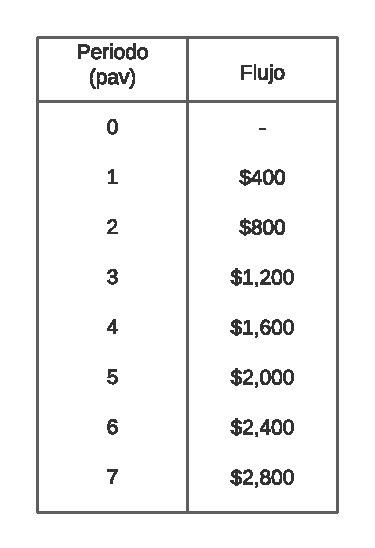
\includegraphics[trim=-5 -5 -5 -5 ,width=0.5\columnwidth]{11/Tabla 1.pdf}} & \multicolumn{1}{|c|}{ 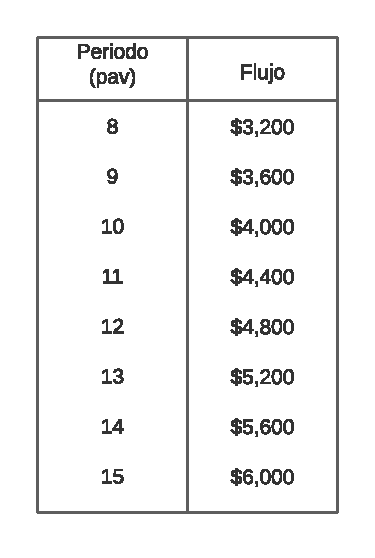
\includegraphics[trim=-5 -5 -5 -5 ,width=0.5\columnwidth]{11/Tabla 2.pdf}} \\ \hline
  \multicolumn{2}{|c|}{\cellcolor[HTML]{FFB183}\textbf{3. Aplicación de funciones}}                                                                                                                  \\ \hline
  \multicolumn{2}{|p{\columnwidth}|}{Se aplicará la función valor presente VNA de la siguiente forma: \newline
  =VNA(0,04;J8::J22) con referencia en la hoja de
  Excel usada para el ejercicio.}                                                                                                                                                                    \\
  \multicolumn{2}{|c|}{ 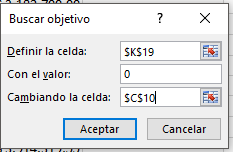
\includegraphics[trim=-5 -5 -5 -5 ,width=0.7\columnwidth]{11/excel1.png}}                                                                                                    \\ \hline
  \multicolumn{2}{|c|}{\cellcolor[HTML]{FFB183}\textbf{4. Gráfica}}                                                                                                                                  \\ \hline
  \multicolumn{2}{|c|}{ \includegraphics[trim=-5 -5 -5 -5 ,width=0.8\columnwidth]{11/gráfico.pdf}}                                                                                                   \\ \hline
  \multicolumn{2}{|c|}{\cellcolor[HTML]{FFB183}\textbf{5. Respuesta}}                                                                                                                                \\ \hline
  \multicolumn{2}{|c|}{El valor presente es VP =  COP 27.697,9410}                                                                                                                                      \\ \hline
 \end{longtable}
 %\newline \newline %USARLO SI CREES QUE ES NECESARIO
\end{center}

	%%%%%%%%%%%%%%%%%%%%%%%%%%FIN EJERCICIO 11 %%%%%%%%%%%%%%%%%%%%%%%%%%%%%%%%%%%%%%%%%%%%%%%%%%%%%%%%%%%%%%%%%%%%%%%%%%%%%%%%%%%%%%%%%%%%%%%%%%%%%%%%%%%%
	
	Observación: el error de  0.02 COP se debe a la aproximación en el valor de la cuota.\\
	
	\section{Capitalización por cuotas con reliquidación de intereses}
	
	Las bases teóricas necesarias para elaborar la tabla son las mismas de la amortización pero poniendo la ecuación en valor final, en consecuencia no entraremos en más detalles.\\
	
	
	
	
	 %%%%%%%%%%%%%%%%%%%%%%%%%%%%%%%%%%%%%%%%%%%%%%%%%%%%%%%%%%%%%%%%%%%%%%%%%%%%%%%%%%%%%%%%%%%%%%%%%%%%%%%%%%%%%%%%%%%%%%%%%%%%%%%%%%%%%%EJERCICIO 12 %%%%%%%%%%%%%%%%%%%%%%%%%%%%%%%%%%%%%%%%%%%%%%%%%%%%%%
	
\textbf{Ejemplo 12}\\
Hallar el valor presente de una serie infinita de egresos que crecen en un 10\%, si la tasa de interés es del 20\% pav y el primer egreso es  300.000COP.\\


%%%%%%%%%%%%%%%%%%% EJERCICIO 12 %%%%%%

%\newpage %USAR SOLO SI EL SOLUCIÓN QUEDA SOLO Y ES NECESARIO BAJARLO A LA SIGUIENTE PAGINA
\textbf{Solución.}\\
%La tabla ira centrada
\begin{center}
	\renewcommand{\arraystretch}{1.6}% Margenes de las celdas
	%Creación de la cuadricula de 3 columnas
	\begin{longtable}[H]{|c|c|c|}
		%Creamos una linea horizontal
		\hline
		%Definimos el color de la primera fila
		\rowcolor[HTML]{FFB183}
		%%%%% INICIO ASIGNACIÓN FECHA FOCAL %%%%%%%
		%%%%%%%%%% INICIO TITULO
		%Lo que se hace aquí es mezclar las 3 columnas en una sola
		\multicolumn{3}{|c|}{\cellcolor[HTML]{FFB183}\textbf{1. Asignación período focal}}  \\ \hline
		\multicolumn{3}{|c|}{$pf = \textit{0 pav}$}   \\\hline
		%%%%%%%%%% FIN TITULO
		%%%%% INICIO DECLARACIÓN DE VARIABLES %%%%%%%
		%%%%%%%%%% INICIO TITULO
		%Lo que se hace aquí es mezclar las 3 columnas en una sola
		\multicolumn{3}{|c|}{\cellcolor[HTML]{FFB183}\textbf{2. Declaración de variables}}   \\ \hline
		%%%%%%%%%% FIN TITULO
		%%%%%%%%%% INICIO DE MATEMÁTICAS
		%Cada & hace referencia al paso de la siguiente columna
		\multicolumn{2}{|c|}{\textbf{$\hspace{3.5 cm}\textit{}\hspace{3.5 cm}$}} & \textbf{$\hspace{3.5 cm}\textit{}\hspace{3.5 cm}$} \\ 
		\multicolumn{2}{|c|}{$\hspace{2 cm}R=  300{.}000COP \hspace{2 cm}$} & $i=20\% \textit{ pav}$ \\
		\multicolumn{2}{|c|}{$\hspace{2 cm}n_1=10  \textit{ pav} \hspace{2 cm}$} & $g=10\% \textit{creciente entre flujos} $ \\
		\multicolumn{2}{|c|}{$\hspace{2 cm}VF= ?COP \hspace{2 cm}$} &  \\ \hline	
		
		%%%%%%%%%% FIN DE MATEMÁTICAS
		%%%%% FIN DECLARACIÓN DE VARIABLES
		
		%%%%% INICIO FLUJO DE CAJA
		\rowcolor[HTML]{FFB183}
		\multicolumn{3}{|c|}{\cellcolor[HTML]{FFB183}\textbf{3. Diagrama de flujo de caja}} \\ \hline
		%Mezclamos 3 columnas y pondremos el dibujo
		%%%%%%%%%%%%% INSERCIÓN DE LA IMAGEN
		%Deberán descargar las imágenes respectivas del drive y pegarlas en la carpeta
		%n_capitulo/img/ejemplos/1/capitulo1ejemplo1.pdf  (el /1/ es el numero del ejemplo)
		\multicolumn{3}{|c|}{ 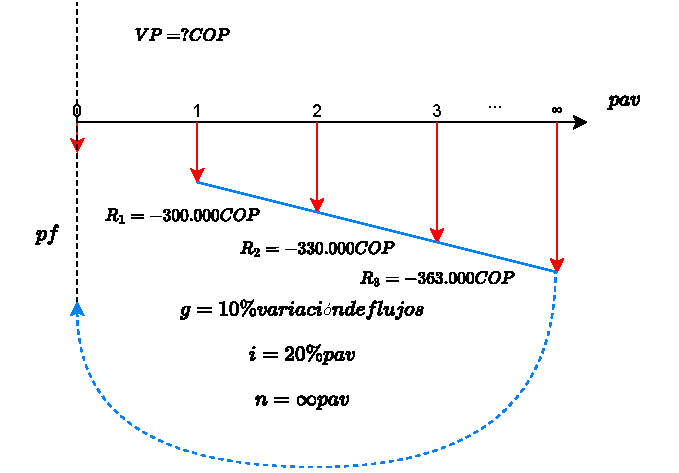
\includegraphics[trim=-5 -5 -5 -5 , scale=0.9]{6_Capitulo/img/ejemplos/12/Capitulo6Ejemplo12.pdf} }
		\\ \hline
		%%%%%%%%%%%%% FIN INSERCIÓN DE IMAGEN
		%%%%%FIN FLUJO DE CAJA
		
		%%%%% INICIO DECLARACIÓN FORMULAS
		%%%%%%%%%%% INICIO TITULO
		\rowcolor[HTML]{FFB183}
		\multicolumn{3}{|c|}{\cellcolor[HTML]{FFB183}\textbf{4. Declaración de fórmulas}}    \\ \hline
		%%%%%%%%%%% FIN TITULO
		%%%%%%%%%%% INICIO MATEMÁTICAS
		\multicolumn{3}{|c|}{$VP=(\frac{R}{i-g}) \hspace{0.4 cm} \textit{Valor gradiente si geométrico infinito si g<1} $} \\   \hline
		
		%%%%%%%%%% FIN MATEMÁTICAS
		%%%%%% INICIO DESARROLLO MATEMÁTICO
		\rowcolor[HTML]{FFB183}
		%%%%%%%%%%INICIO TITULO
		\multicolumn{3}{|c|}{\cellcolor[HTML]{FFB183}\textbf{5. Desarrollo matemático}}       \\ \hline
		%%%%%%%%%% FIN TITULO
		%%%%%%%%%% INICIO MATEMÁTICAS
		\multicolumn{3}{|c|}{$VP=(\frac{  300{.}000COP}{0.2-0.1}) \hspace{0.2 cm}\rightarrow \hspace{0.2 cm} VP= 300{.}000 COP$} \\  \hline
		%%%%%%%%%% FIN MATEMÁTICAS
		%%%%%% FIN DESARROLLO MATEMÁTICO
		%%%%%% INICIO RESPUESTA
		\rowcolor[HTML]{FFB183}
		%%%%%%%%%%INICIO TITULO
		\multicolumn{3}{|c|}{\cellcolor[HTML]{FFB183}\textbf{6. Respuesta}}   \\ \hline
		%%%%%%%%%% FIN TITULO
		%%%%%%%%%% INICIO RESPUESTA MATEMÁTICA
		\multicolumn{3}{|c|}{${VP=  300.000 COP }$} \\ \hline
		%%%%%%%%%% FIN MATEMÁTICAS
		%%%%%% FIN RESPUESTA
	\end{longtable}
	%Se crean dos lineas en blanco para que no quede el siguiente texto tan pegado
	%\newline \newline %USARLO SI CREES QUE ES NECESARIO
\end{center}

%%%%%%%%%%%%%%%%%%%%%%%%%%FIN EJERCICIO 12 %%%%%%%%%%%%%%%%%%%%%%%%%%%

	%%%%%%%%%%%%%%%%%%%%%%%%%%FIN EJERCICIO 12 %%%%%%%%%%%%%%%%%%%%%%%%%%%%%%%%%%%%%%%%%%%%%%%%%%%%%%%%%%%%%%%%%%%%%%%%%%%%%%%%%%%%%%%%%%%%%%%%%%%%%%%%%%%%
	
	
	
	\section{Costo periódico de una deuda}
	
	Cuando el fondo está destinado a cancelar una deuda y los depósitos en el fondo son uniformes entonces se denomina costo periódico de una deuda a la cantidad que debemos disponer en cada período para pagar los intereses de la deuda y hacer el depósito correspondiente en el fondo. Según la duración del período, se dice que la deuda tiene un costo trimestral, mensual, etc.\\
	
	\begin{comment}
	\textbf{Ejemplo 19}\\
	Supongamos que tenemos que pagar la suma de  COP  800.000 al final de 2 años y mientras tanto debemos pagar intereses a la tasa del 3\% mensual vencido. Con el fin de ir reuniendo el dinero necesario para cancelar la deuda se constituye un fondo mediante depósitos mensuales iguales que ganan un interés del 2.5\% efectivo mensual. Calcular el costo mensual de la deuda.\\
	
	\textbf{Solución:}\\
	\textbf{a.}	Diagrama de flujo de caja:
	\begin{center}
		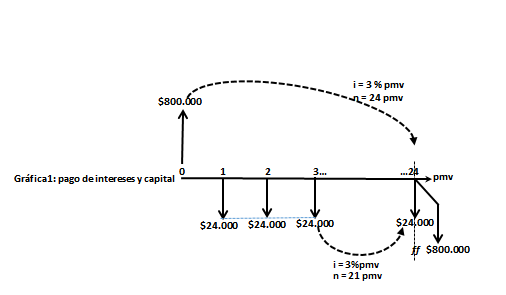
\includegraphics[height=9cm]{7_48}
	\end{center}
	\\
	\begin{center}
		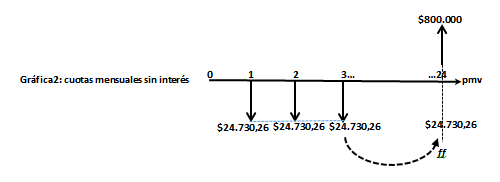
\includegraphics[height=6cm]{7_49}
	\end{center}
	
	Mensualmente debemos pagar un interés de  COP  800.000 x 0,03 =  COP  24.000
	Por otra parte, el depósito mensual en el fondo será:
	 COP  800.000 = Rx24 (1,025); \\R =   COP  24.730,26
	Y el costo mensual de la deuda será: 24.000 + 24.730,26 =  COP  48.730,26\\
	
	\textbf{b.}	Respuesta:\\
	La primera gráfica representa el pago de intereses y la deuda, la segunda gráfica representa los depósitos en el fondo y el capital reunido, al final de los 2 años se cancela el fondo y con ese dinero se paga la deuda.\\
	
	\textbf{Observación:} cuando la capitalización se hace mediante cuotas crecientes, por ejemplo con un gradiente, entonces el costo de la deuda de cada período es variable.\\
	\end{comment}
	%\textbf{Ejemplo 20}\\
	
	%%%%%%%%%%%%%%%%%%%%%%%%%%%%%%%%%%%%%%%%%%%%%%%%%%%%%%%%%%%%%%%%%%%%%%%%%%%%%%%%%%%%%%%%%%%%%%%%%%%%%%%%%%%%
	
	%%%%%%%%%%%%%%%%%%%%%%%%%%EJERCICIO 13 %%%%%%%%%%%%%%%%%%%%%%%%%%%%%%%%%%%%%%%%%%%%%%%%%%%%%%
		%%%%%%%%%%%%%%%%%%%%%%%%%%EJERCICIO 13 %%%%%%%%%%%%%%%%%%%%%%%%%%%%%%%%%%%%%%%%%%%%%%%%%%%%%%
    \textbf{Ejemplo 13}\\
	
	Una cuota inicial del 30\% y el saldo será pagadero al final de 3 años, mientras tanto se pagarán intereses por período mes anticipado al 3\%. Con el objeto de cancelar la deuda a su vencimiento, se constituye un fondo que paga el 33\% nominal anual mes vencido mediante depósitos mensuales ordinarios crecientes en 2.000 COP. Determinar el costo del período 15.\\
	
	\textbf{Solución 13}\\
	%La tabla ira centrada
	\begin{center}
		\renewcommand{\arraystretch}{1.5}% Margenes de las celdas
		%Creación de la cuadricula de 3 columnas
		\begin{longtable}[H]{|p{0.5\linewidth}|p{0.5\linewidth}|}
			%Creamos una linea horizontal
			\hline
			%Definimos el color de la primera fila
			\rowcolor[HTML]{FFB183}
			%%%%% INICIO ASIGNACIÓN período FOCAL %%%%%%%
			%%%%%%%%%% INICIO TITULO
			%Lo que se hace aquí es mezclar las 3 columnas en una sola
			\multicolumn{2}{|c|}{\cellcolor[HTML]{FFB183}\textbf{1. Asignación período focal}}   \\ \hline
			%%%%%%%%%% FIN TITULO
			%%%%% INICIO DECLARACIÓN DE VARIABLES %%%%%%%
			\multicolumn{2}{|c|}{$pf = 36 \textit{ pmv}$}\\ \hline
			%%%%%%%%%% INICIO TITULO
			%Lo que se hace aquí es mezclar las 3 columnas en una sola
			\multicolumn{2}{|c|}{\cellcolor[HTML]{FFB183}\textbf{2. Declaración de variables}}   \\ \hline
			%%%%%%%%%% FIN TITULO
			%%%%%%%%%% INICIO DE MATEMÁTICAS
			%Cada & hace referencia al paso de la siguiente columna
			$  Interés = 4.200.000 \ COP (0,03) = 126.000 \ COP $  			 \\ \hline
			%%%%%%%%%% FIN DE MATEMÁTICAS
			%%%%% FIN DECLARACIÓN DE VARIABLES
			
			\rowcolor[HTML]{FFB183}
			\multicolumn{2}{|c|}{\cellcolor[HTML]{FFB183}\textbf{3. Diagrama de flujo de caja}} \\ \hline
			\multicolumn{2}{|c|}{ 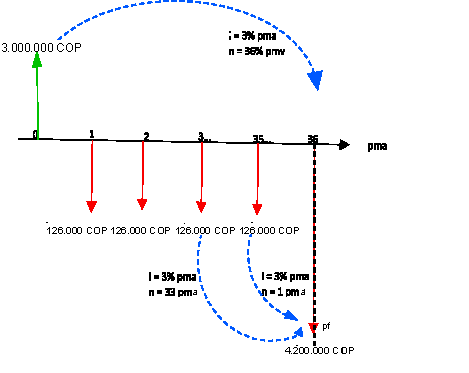
\includegraphics[trim=-78 -5 -78 -5]{7_Capitulo/img/ejemplos/13/13_1.pdf} }   \\
			\multicolumn{2}{|c|}{ 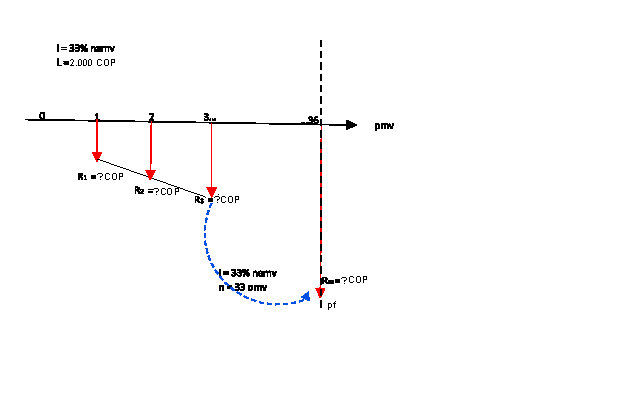
\includegraphics[trim=-78 -5 -78 -5]{7_Capitulo/img/ejemplos/13/13_2.pdf} }   \\ \hline
			%%%%% INICIO FLUJO DE CAJA
			\rowcolor[HTML]{FFB183}
			\multicolumn{2}{|c|}{\cellcolor[HTML]{FFB183}\textbf{4. Declaración de fórmulas}} \\ \hline
			%%%%%%%%%%%%% FIN INSERCIÓN DE IMAGEN
			%%%%%FIN FLUJO DE CAJA
			\multicolumn{2}{|c|}{ $VF = R n(1+i)^{n-1} $ \hspace{1mm} Formula del valor futuro gradiente geométrico si g=i}\\    
			\multicolumn{2}{|c|}{ $R_{n} = R_{1} + (n-1)L $ \hspace{1mm} Valor de un periodo aritmetico en un periodo n}   \\ \hline
			
			%%%%%% INICIO DESARROLLO MATEMÁTICO
			\rowcolor[HTML]{FFB183}
			%%%%%%%%%%INICIO TITULO
			\multicolumn{2}{|c|}{\cellcolor[HTML]{FFB183}\textbf{5. Desarrollo matemático}}       \\ \hline
			%%%%%%%%%% FIN TITULO
			%%%%%%%%%% INICIO MATEMÁTICAS
			\multicolumn{2}{|c|}{  $ 4.200.000 \ COP = R_{1} (36) (0,0275) + \frac{ 2.000 \ COP }{0,0275} ((36)(0,0275)-36) $}   \\ 
			\multicolumn{2}{|c|}{  $  R_{1} = 40.531,73 \ COP $}   \\ 
			\multicolumn{2}{|c|}{ $  R_{15} = 40.531,73 \ COP +  ( 15 - 1) (2.000 \ COP) = 68.531,73 \ COP $}   \\  \hline
			
			%%%%%%%%%% FIN MATEMÁTICAS
			%%%%%% FIN DESARROLLO MATEMÁTICO
			%%%%%% INICIO RESPUESTA
			\rowcolor[HTML]{FFB183}
			%%%%%%%%%%INICIO TITULO
			\multicolumn{2}{|c|}{\cellcolor[HTML]{FFB183}\textbf{6. Respuesta}}   \\ \hline
			%%%%%%%%%% FIN TITULO
			%%%%%%%%%% INICIO RESPUESTA MATEMÁTICA
			%\multicolumn{2}{|c|}{ 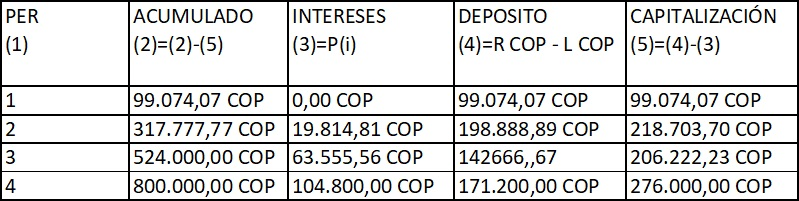
\includegraphics[trim=-78 -5 -78 -5]{7_Capitulo/img/ejemplos/12/12_2.jpg} }   \\ \hline
			\multicolumn{2}{|C{\textwidth}|}{
				$  R_{1} = 40.531,73 \ COP \hspace{2mm} y  \hspace{2mm} R_{15} = 68.531,73 \ COP $
				
				Esto significa que en el período 15 el deudor debe disponer de 194.531,73 COP de los cuales 126.000 COP los dedica al pago de intereses y el resto (68.531,73 COP) se deposita en el fondo.
				
			}  \\ \hline
			
			
			%%%%%%%%%% FIN MATEMÁTICAS
			%%%%%% FIN RESPUESTA
		\end{longtable}
		%Se crean dos lineas en blanco para que no quede el siguiente texto tan pegado
		%\newline \newline %USARLO SI CREES QUE ES NECESARIO
	\end{center}
%%%%%%%%%%%%%%%%%%%%%%%%%%FIN EJERCICIO 13
	%%%%%%%%%%%%%%%%%%%%%%%%%%FIN EJERCICIO 13
	
	
